\documentclass[12pt,oneside]{report}

% Load preamble
\newcommand{\course}[1]{\newcommand{\courseloc}{#1}}

\usepackage{amsmath,amssymb,amsfonts,mathtools,amsthm}
\usepackage{mathrsfs}
\usepackage{booktabs, emptypage, subcaption, multicol}
\usepackage{braket, bm, lipsum, systeme}
\usepackage{hyperref,theoremref}
\hypersetup{
  pdftitle={assignment},
  colorlinks=true, linkcolor=doc!90,
  bookmarksnumbered=true,
  bookmarksopen=true
}
\usepackage[T1]{fontenc}
\usepackage{anyfontsize}
\usepackage{lmodern}
\usepackage{graphicx}
\usepackage{import}
\usepackage{transparent}
\usepackage{float}
\usepackage[tmargin=2cm,rmargin=1in,lmargin=1in,margin=0.85in,bmargin=2cm,footskip=.4in]{geometry}
\usepackage[shortlabels]{enumitem}
\usepackage[dvipsnames]{xcolor}
\usepackage{xfrac}
\usepackage{comment}
\let\mathbf\relax
\usepackage[varbb]{newpxmath}
\usepackage[most,many,breakable]{tcolorbox}
\usepackage{varwidth}
\usepackage{nameref}
\usepackage[ruled,vlined,linesnumbered]{algorithm2e}
\usepackage{chngcntr}
\usepackage{import}
\usepackage{xifthen}
\usepackage{pdfpages}
\usepackage{transparent}
\usepackage{xparse}
\usepackage{pgffor}
%\usepackage{emoji}
\usepackage{stmaryrd}
\usepackage{listings}
\usepackage{siunitx}
\usepackage{tikz, tikz-cd, tikz-3dplot, tikzsymbols}
\usetikzlibrary{intersections, angles, quotes, calc, positioning, arrows.meta}
\usepackage{pgfplots}
\pgfplotsset{compat=1.13}
\usepackage{thmtools}
\usepackage[framemethod=TikZ]{mdframed}
\usepackage{etoolbox}
\usepackage{xifthen} 
\usepackage{titlesec}
\usepackage[dotinlabels]{titletoc}
\usepackage{fancyhdr}
\usepackage{marginnote}
\usepackage{witharrows}
\usepackage{scalerel}
\usepackage[usestackEOL]{stackengine}
\usepackage[linguistics]{forest}
\usepackage{array}
\usepackage[export]{adjustbox}
\usepackage{multirow}
\usepackage{tabularx}
\usepackage{extarrows}
\usepackage[ 
backend=biber,
backref=true,
style=numeric,
sortcites=true,
sorting=none,
defernumbers=true
]{biblatex}
\usepackage{xurl}
\usepackage[makeroom]{cancel}
\usepackage{bookmark}
\usepackage{tensor}
\usepackage{derivative}
\usepackage{annotate-equations}
\usepackage{dashbox}
\usepackage{nicematrix}
\usepackage{ytableau}
\usepackage{tabularray}
\usepackage{xpatch}





%=================================
%= TikZ things customized        =
%=================================


\newcommand\mycommfont[1]{\footnotesize\ttfamily\textcolor{blue}{#1}}
\SetCommentSty{mycommfont}
\newcommand{\incfig}[2]{%
    \def\svgwidth{#1\columnwidth}
    \import{./figures/}{#2.pdf_tex}
}

\graphicspath{{./figures/}}
\pdfsuppresswarningpagegroup=1







\usepackage{tikzsymbols}
\tikzset{
	symbol/.style={
			draw=none,
			every to/.append style={
					edge node={node [sloped, allow upside down, auto=false]{$#1$}}}
		}
}
\tikzstyle{c} = [circle,fill=black,scale=0.5]
\tikzstyle{b} = [draw, thick, black, -]
\tikzset{
    vertex/.style={
        circle,
        draw,
        minimum size=6mm,
        inner sep=0pt
    }
}

%\tikzset{
%    force/.style={thick, {Circle[length=2pt]}-stealth, shorten <=-1pt}
%}

%%%%%%%%%%%%%%%%%%%%%%%%%%%%%%
% SELF MADE COLORS
%%%%%%%%%%%%%%%%%%%%%%%%%%%%%%

\definecolor{doc}{RGB}{0,60,110}
\definecolor{myg}{RGB}{56, 140, 70}
\definecolor{myb}{RGB}{45, 111, 177}
\definecolor{myr}{RGB}{199, 68, 64}
\definecolor{mytheorembg}{HTML}{F2F2F9}
\definecolor{mytheoremfr}{HTML}{00007B}
\definecolor{mylemmabg}{HTML}{FFFAF8}
\definecolor{mylemmafr}{HTML}{983b0f}
\definecolor{mypropbg}{HTML}{f2fbfc}
\definecolor{mypropfr}{HTML}{191971}
\definecolor{myexamplebg}{HTML}{F2FBF8}
\definecolor{myexamplefr}{HTML}{88D6D1}
\definecolor{myexampleti}{HTML}{2A7F7F}
\definecolor{mydefinitbg}{HTML}{E5E5FF}
\definecolor{mydefinitfr}{HTML}{3F3FA3}
\definecolor{notesgreen}{RGB}{0,162,0}
\definecolor{myp}{RGB}{197, 92, 212}
\definecolor{mygr}{HTML}{2C3338}
\definecolor{myred}{RGB}{127,0,0}
\definecolor{myyellow}{RGB}{169,121,69}
\definecolor{myexercisebg}{HTML}{F2FBF8}
\definecolor{myexercisefg}{HTML}{88D6D1}

%%%%%%%%%%%%%%%%%%%%%%%%%%%%
% TCOLORBOX SETUPS
%%%%%%%%%%%%%%%%%%%%%%%%%%%%

\setlength{\parindent}{1cm}
%================================
% THEOREM BOX
%================================

\tcbuselibrary{theorems,skins,hooks}
\newtcbtheorem[number within=section]{Theorem}{Theorem}
{%
	enhanced,
	breakable,
	colback = mytheorembg,
	frame hidden,
	boxrule = 0sp,
	borderline west = {2pt}{0pt}{mytheoremfr},
	sharp corners,
	detach title,
	before upper = \tcbtitle\par\smallskip,
	coltitle = mytheoremfr,
	fonttitle = \bfseries\sffamily,
	description font = \mdseries,
	separator sign none,
	segmentation style={solid, mytheoremfr},
}
{th}

\newtcbtheorem[number within=chapter]{theorem}{Theorem}
{%
	enhanced,
	breakable,
	colback = mytheorembg,
	frame hidden,
	boxrule = 0sp,
	borderline west = {2pt}{0pt}{mytheoremfr},
	sharp corners,
	detach title,
	before upper = \tcbtitle\par\smallskip,
	coltitle = mytheoremfr,
	fonttitle = \bfseries\sffamily,
	description font = \mdseries,
	separator sign none,
	segmentation style={solid, mytheoremfr},
}
{th}


\newtcolorbox{Theoremcon}
{%
	enhanced
	,breakable
	,colback = mytheorembg
	,frame hidden
	,boxrule = 0sp
	,borderline west = {2pt}{0pt}{mytheoremfr}
	,sharp corners
	,description font = \mdseries
	,separator sign none
}

%================================
% Corollery
%================================
\newtcbtheorem[number within=section]{Corollary}{Corollary}
{%
	enhanced
	,breakable
	,colback = myp!10
	,frame hidden
	,boxrule = 0sp
	,borderline west = {2pt}{0pt}{myp!85!black}
	,sharp corners
	,detach title
	,before upper = \tcbtitle\par\smallskip
	,coltitle = myp!85!black
	,fonttitle = \bfseries\sffamily
	,description font = \mdseries
	,separator sign none
	,segmentation style={solid, myp!85!black}
}
{th}
\newtcbtheorem[number within=chapter]{corollary}{Corollary}
{%
	enhanced
	,breakable
	,colback = myp!10
	,frame hidden
	,boxrule = 0sp
	,borderline west = {2pt}{0pt}{myp!85!black}
	,sharp corners
	,detach title
	,before upper = \tcbtitle\par\smallskip
	,coltitle = myp!85!black
	,fonttitle = \bfseries\sffamily
	,description font = \mdseries
	,separator sign none
	,segmentation style={solid, myp!85!black}
}
{th}


%================================
% LEMMA
%================================

\newtcbtheorem[number within=section]{Lemma}{Lemma}
{%
	enhanced,
	breakable,
	colback = mylemmabg,
	frame hidden,
	boxrule = 0sp,
	borderline west = {2pt}{0pt}{mylemmafr},
	sharp corners,
	detach title,
	before upper = \tcbtitle\par\smallskip,
	coltitle = mylemmafr,
	fonttitle = \bfseries\sffamily,
	description font = \mdseries,
	separator sign none,
	segmentation style={solid, mylemmafr},
}
{th}

\newtcbtheorem[number within=chapter]{lemma}{lemma}
{%
	enhanced,
	breakable,
	colback = mylemmabg,
	frame hidden,
	boxrule = 0sp,
	borderline west = {2pt}{0pt}{mylemmafr},
	sharp corners,
	detach title,
	before upper = \tcbtitle\par\smallskip,
	coltitle = mylemmafr,
	fonttitle = \bfseries\sffamily,
	description font = \mdseries,
	separator sign none,
	segmentation style={solid, mylemmafr},
}
{th}

%================================
% Exercise
%================================

\newtcbtheorem[number within=section]{Exercise}{Exercise}
{%
	enhanced,
	breakable,
	colback = myexercisebg,
	frame hidden,
	boxrule = 0sp,
	borderline west = {2pt}{0pt}{myexercisefg},
	sharp corners,
	detach title,
	before upper = \tcbtitle\par\smallskip,
	coltitle = myexercisefg,
	fonttitle = \bfseries\sffamily,
	description font = \mdseries,
	separator sign none,
	segmentation style={solid, myexercisefg},
}
{th}

\newtcbtheorem[number within=chapter]{exercise}{Exercise}
{%
	enhanced,
	breakable,
	colback = myexercisebg,
	frame hidden,
	boxrule = 0sp,
	borderline west = {2pt}{0pt}{myexercisefg},
	sharp corners,
	detach title,
	before upper = \tcbtitle\par\smallskip,
	coltitle = myexercisefg,
	fonttitle = \bfseries\sffamily,
	description font = \mdseries,
	separator sign none,
	segmentation style={solid, myexercisefg},
}
{th}


%================================
% PROPOSITION
%================================

\newtcbtheorem[number within=section]{Prop}{Proposition}
{%
	enhanced,
	breakable,
	colback = mypropbg,
	frame hidden,
	boxrule = 0sp,
	borderline west = {2pt}{0pt}{mypropfr},
	sharp corners,
	detach title,
	before upper = \tcbtitle\par\smallskip,
	coltitle = mypropfr,
	fonttitle = \bfseries\sffamily,
	description font = \mdseries,
	separator sign none,
	segmentation style={solid, mypropfr},
}
{th}

\newtcbtheorem[number within=chapter]{prop}{Proposition}
{%
	enhanced,
	breakable,
	colback = mypropbg,
	frame hidden,
	boxrule = 0sp,
	borderline west = {2pt}{0pt}{mypropfr},
	sharp corners,
	detach title,
	before upper = \tcbtitle\par\smallskip,
	coltitle = mypropfr,
	fonttitle = \bfseries\sffamily,
	description font = \mdseries,
	separator sign none,
	segmentation style={solid, mypropfr},
}
{th}


%================================
% CLAIM
%================================

\newtcbtheorem[number within=section]{claim}{Claim}
{%
	enhanced
	,breakable
	,colback = myg!10
	,frame hidden
	,boxrule = 0sp
	,borderline west = {2pt}{0pt}{myg}
	,sharp corners
	,detach title
	,before upper = \tcbtitle\par\smallskip
	,coltitle = myg!85!black
	,fonttitle = \bfseries\sffamily
	,description font = \mdseries
	,separator sign none
	,segmentation style={solid, myg!85!black}
}
{th}



%================================
% EXAMPLE BOX
%================================

\newtcbtheorem[number within=section]{Example}{Example}
{%
	colback = myexamplebg
	,breakable
	,colframe = myexamplefr
	,coltitle = myexampleti
	,boxrule = 1pt
	,sharp corners
	,detach title
	,before upper=\tcbtitle\par\smallskip
	,fonttitle = \bfseries
	,description font = \mdseries
	,separator sign none
	,description delimiters parenthesis
}
{ex}

\newtcbtheorem[number within=chapter]{example}{Example}
{%
	colback = myexamplebg
	,breakable
	,colframe = myexamplefr
	,coltitle = myexampleti
	,boxrule = 1pt
	,sharp corners
	,detach title
	,before upper=\tcbtitle\par\smallskip
	,fonttitle = \bfseries
	,description font = \mdseries
	,separator sign none
	,description delimiters parenthesis
}
{ex}

%================================
% DEFINITION BOX
%================================

\newtcbtheorem[number within=section]{Definition}{Definition}{enhanced,
	before skip=2mm,after skip=2mm, colback=red!5,colframe=red!80!black,boxrule=0.5mm,
	attach boxed title to top left={xshift=1cm,yshift*=1mm-\tcboxedtitleheight}, varwidth boxed title*=-3cm,
	boxed title style={frame code={
					\path[fill=tcbcolback]
					([yshift=-1mm,xshift=-1mm]frame.north west)
					arc[start angle=0,end angle=180,radius=1mm]
					([yshift=-1mm,xshift=1mm]frame.north east)
					arc[start angle=180,end angle=0,radius=1mm];
					\path[left color=tcbcolback!60!black,right color=tcbcolback!60!black,
						middle color=tcbcolback!80!black]
					([xshift=-2mm]frame.north west) -- ([xshift=2mm]frame.north east)
					[rounded corners=1mm]-- ([xshift=1mm,yshift=-1mm]frame.north east)
					-- (frame.south east) -- (frame.south west)
					-- ([xshift=-1mm,yshift=-1mm]frame.north west)
					[sharp corners]-- cycle;
				},interior engine=empty,
		},
	fonttitle=\bfseries,
	title={#2},#1}{def}
\newtcbtheorem[number within=chapter]{definition}{Definition}{enhanced,
	before skip=2mm,after skip=2mm, colback=red!5,colframe=red!80!black,boxrule=0.5mm,
	attach boxed title to top left={xshift=1cm,yshift*=1mm-\tcboxedtitleheight}, varwidth boxed title*=-3cm,
	boxed title style={frame code={
					\path[fill=tcbcolback]
					([yshift=-1mm,xshift=-1mm]frame.north west)
					arc[start angle=0,end angle=180,radius=1mm]
					([yshift=-1mm,xshift=1mm]frame.north east)
					arc[start angle=180,end angle=0,radius=1mm];
					\path[left color=tcbcolback!60!black,right color=tcbcolback!60!black,
						middle color=tcbcolback!80!black]
					([xshift=-2mm]frame.north west) -- ([xshift=2mm]frame.north east)
					[rounded corners=1mm]-- ([xshift=1mm,yshift=-1mm]frame.north east)
					-- (frame.south east) -- (frame.south west)
					-- ([xshift=-1mm,yshift=-1mm]frame.north west)
					[sharp corners]-- cycle;
				},interior engine=empty,
		},
	fonttitle=\bfseries,
	title={#2},#1}{def}


%================================
% EXERCISE BOX
%================================

\newcounter{questioncounter}
\counterwithin{questioncounter}{chapter}
% \counterwithin{questioncounter}{section}

\makeatletter
\newtcbtheorem[use counter=questioncounter]{question}{Question}{enhanced,
	breakable,
	colback=white,
	colframe=myb!80!black,
	attach boxed title to top left={yshift*=-\tcboxedtitleheight},
	fonttitle=\bfseries,
	title={#2},
	boxed title size=title,
	boxed title style={%
			sharp corners,
			rounded corners=northwest,
			colback=tcbcolframe,
			boxrule=0pt,
		},
	underlay boxed title={%
			\path[fill=tcbcolframe] (title.south west)--(title.south east)
			to[out=0, in=180] ([xshift=5mm]title.east)--
			(title.center-|frame.east)
			[rounded corners=\kvtcb@arc] |-
			(frame.north) -| cycle;
		},
	#1
}{def}
\makeatother

%================================
% SOLUTION BOX
%================================

\makeatletter
\newtcolorbox{solution}{enhanced,
	breakable,
	colback=white,
	colframe=myg!80!black,
	attach boxed title to top left={yshift*=-\tcboxedtitleheight},
	title=Solution,
	boxed title size=title,
	boxed title style={%
			sharp corners,
			rounded corners=northwest,
			colback=tcbcolframe,
			boxrule=0pt,
		},
	underlay boxed title={%
			\path[fill=tcbcolframe] (title.south west)--(title.south east)
			to[out=0, in=180] ([xshift=5mm]title.east)--
			(title.center-|frame.east)
			[rounded corners=\kvtcb@arc] |-
			(frame.north) -| cycle;
		},
}
\makeatother

%================================
% Question BOX
%================================

\makeatletter
\newtcbtheorem{qstion}{Question}{enhanced,
	breakable,
	colback=white,
	colframe=mygr,
	attach boxed title to top left={yshift*=-\tcboxedtitleheight},
	fonttitle=\bfseries,
	title={#2},
	boxed title size=title,
	boxed title style={%
			sharp corners,
			rounded corners=northwest,
			colback=tcbcolframe,
			boxrule=0pt,
		},
	underlay boxed title={%
			\path[fill=tcbcolframe] (title.south west)--(title.south east)
			to[out=0, in=180] ([xshift=5mm]title.east)--
			(title.center-|frame.east)
			[rounded corners=\kvtcb@arc] |-
			(frame.north) -| cycle;
		},
	#1
}{def}
\makeatother

\newtcbtheorem[number within=chapter]{wconc}{Wrong Concept}{
	breakable,
	enhanced,
	colback=white,
	colframe=myr,
	arc=0pt,
	outer arc=0pt,
	fonttitle=\bfseries\sffamily\large,
	colbacktitle=myr,
	attach boxed title to top left={},
	boxed title style={
			enhanced,
			skin=enhancedfirst jigsaw,
			arc=3pt,
			bottom=0pt,
			interior style={fill=myr}
		},
	#1
}{def}


%================================
% NOTE BOX
%================================

\usetikzlibrary{arrows,calc,shadows.blur}
\tcbuselibrary{skins}
\newtcolorbox{note}[1][]{%
	enhanced jigsaw,
	colback=gray!20!white,%
	colframe=gray!80!black,
	size=small,
	boxrule=1pt,
	title=\textbf{Note:-},
	halign title=flush center,
	coltitle=black,
	breakable,
	drop shadow=black!50!white,
	attach boxed title to top left={xshift=1cm,yshift=-\tcboxedtitleheight/2,yshifttext=-\tcboxedtitleheight/2},
	minipage boxed title=1.5cm,
	boxed title style={%
			colback=white,
			size=fbox,
			boxrule=1pt,
			boxsep=2pt,
			underlay={%
					\coordinate (dotA) at ($(interior.west) + (-0.5pt,0)$);
					\coordinate (dotB) at ($(interior.east) + (0.5pt,0)$);
					\begin{scope}
						\clip (interior.north west) rectangle ([xshift=3ex]interior.east);
						\filldraw [white, blur shadow={shadow opacity=60, shadow yshift=-.75ex}, rounded corners=2pt] (interior.north west) rectangle (interior.south east);
					\end{scope}
					\begin{scope}[gray!80!black]
						\fill (dotA) circle (2pt);
						\fill (dotB) circle (2pt);
					\end{scope}
				},
		},
	#1,
}



%%%%%%%%%%%%%%%%%%%%%%%%%%%%%%
%  TITLE BOX FOR PSETS 
%%%%%%%%%%%%%%%%%%%%%%%%%%%%%%

\newtcolorbox{titlebox}[1][]{%
	enhanced jigsaw,
	colback=gray!20!white,%
	colframe=gray!80!black,
	boxrule=1pt,
	title=\textbf{#1},
	halign title=flush center,
	coltitle=black,
	breakable,
	drop shadow=black!50!white,
	attach boxed title to top left={xshift=1cm,yshift=-\tcboxedtitleheight/2,yshifttext=-\tcboxedtitleheight/2},
	minipage boxed title=4cm,
	sidebyside,
	sidebyside align=top,
	lefthand ratio=0.55,
	boxed title style={%
			colback=white,
			size=fbox,
			boxrule=1pt,
			boxsep=2pt,
			underlay={%
					\coordinate (dotA) at ($(interior.west) + (-0.5pt,0)$);
					\coordinate (dotB) at ($(interior.east) + (0.5pt,0)$);
					\begin{scope}
						\clip (interior.north west) rectangle ([xshift=3ex]interior.east);
						\filldraw [white, blur shadow={shadow opacity=60, shadow yshift=-.75ex}, rounded corners=2pt] (interior.north west) rectangle (interior.south east);
					\end{scope}
					\begin{scope}[gray!80!black]
						\fill (dotA) circle (2pt);
						\fill (dotB) circle (2pt);
					\end{scope}
				},
		},
}









%%%%%%%%%%%%%%%%%%%%%%%%%%%%%%
% SELF MADE COMMANDS
%%%%%%%%%%%%%%%%%%%%%%%%%%%%%%

\newcommand{\thm}[2]{\begin{Theorem}{#1}{}#2\end{Theorem}}
\newcommand{\cor}[2]{\begin{Corollary}{#1}{}#2\end{Corollary}}
\newcommand{\mlemma}[2]{\begin{Lemma}{#1}{}#2\end{Lemma}}
\newcommand{\mer}[2]{\begin{Exercise}{#1}{}#2\end{Exercise}}
\newcommand{\mprop}[2]{\begin{Prop}{#1}{}#2\end{Prop}}
\newcommand{\clm}[3]{\begin{claim}{#1}{#2}#3\end{claim}}
\newcommand{\wc}[2]{\begin{wconc}{#1}{}\setlength{\parindent}{1cm}#2\end{wconc}}
\newcommand{\thmcon}[1]{\begin{Theoremcon}{#1}\end{Theoremcon}}
\newcommand{\ex}[2]{\begin{Example}{#1}{}#2\end{Example}}
\newcommand{\dfn}[2]{\begin{Definition}[colbacktitle=red!75!black]{#1}{}#2\end{Definition}}
\newcommand{\dfnc}[2]{\begin{definition}[colbacktitle=red!75!black]{#1}{}#2\end{definition}}
\newcommand{\qs}[2]{\begin{question}{#1}{}#2\end{question}}
\newcommand{\pf}[2]{\begin{myproof}[#1]#2\end{myproof}}
\newcommand{\nt}[1]{\begin{note}#1\end{note}}

\newcommand*\circled[1]{\tikz[baseline=(char.base)]{
		\node[shape=circle,draw,inner sep=1pt] (char) {#1};}}
\newcommand\getcurrentref[1]{%
	\ifnumequal{\value{#1}}{0}
	{??}
	{\the\value{#1}}%
}
\newcommand{\getCurrentSectionNumber}{\getcurrentref{section}}
\newenvironment{myproof}[1][\proofname]{%
	\proof[\bfseries #1: ]%
}{\endproof}

\newcommand{\mclm}[2]{\begin{myclaim}[#1]#2\end{myclaim}}
\newenvironment{myclaim}[1][\claimname]{\proof[\bfseries #1: ]}{}
\newenvironment{iclaim}[1][\claimname]{\bfseries #1\mdseries:}{}
\newcommand{\iclm}[2]{\begin{iclaim}[#1]#2\end{iclaim}}

\newcounter{mylabelcounter}

\makeatletter
\newcommand{\setword}[2]{%
	\phantomsection
	#1\def\@currentlabel{\unexpanded{#1}}\label{#2}%
}
\makeatother

% deliminators

\newsavebox\diffdbox
\newcommand{\slantedromand}{{\mathpalette\makesl{d}}}
\newcommand{\makesl}[2]{%
\begingroup
\sbox{\diffdbox}{$\mathsurround=0pt#1\mathrm{#2}$}%
\pdfsave
\pdfsetmatrix{1 0 0.2 1}%
\rlap{\usebox{\diffdbox}}%
\pdfrestore
\hskip\wd\diffdbox
\endgroup
}
\newcommand{\dd}[1][]{\ensuremath{\mathop{}\!\ifstrempty{#1}{%
\slantedromand\@ifnextchar^{\hspace{0.2ex}}{\hspace{0.1ex}}}%
{\slantedromand\hspace{0.2ex}^{#1}}}}
\ProvideDocumentCommand\dv{o m g}{%
  \ensuremath{%
    \IfValueTF{#3}{%
      \IfNoValueTF{#1}{%
        \frac{\dd #2}{\dd #3}%
      }{%
        \frac{\dd^{#1} #2}{\dd #3^{#1}}%
      }%
    }{%
      \IfNoValueTF{#1}{%
        \frac{\dd}{\dd #2}%
      }{%
        \frac{\dd^{#1}}{\dd #2^{#1}}%
      }%
    }%
  }%
}
\providecommand*{\pdv}[3][]{\frac{\partial^{#1}#2}{\partial#3^{#1}}}
%  - others
\DeclareMathOperator{\Lap}{\mathcal{L}}
\DeclareMathOperator{\Var}{Var} % varience
\DeclareMathOperator{\Cov}{Cov} % covarience
\DeclareMathOperator{\E}{E} % expected

% Since the amsthm package isn't loaded

% I prefer the slanted \leq
\let\oldleq\leq % save them in case they're every wanted
\let\oldgeq\geq
\renewcommand{\leq}{\leqslant}
\renewcommand{\geq}{\geqslant}

%%%%%%%%%%%%%%%%%%%%%%%%%%%%%%%%%%%%%%%%%%%
% TABLE OF CONTENTS
%%%%%%%%%%%%%%%%%%%%%%%%%%%%%%%%%%%%%%%%%%%

\contentsmargin{0cm}
\titlecontents{chapter}[3.7pc]
{\addvspace{30pt}%
	\begin{tikzpicture}[remember picture, overlay]%
		\draw[fill=doc!60,draw=doc!60] (-7,-.1) rectangle (-0.9,.5);%
		\pgftext[left,x=-3.7cm,y=0.2cm]{\color{white}\Large\sc\bfseries Chapter\ \thecontentslabel};%
	\end{tikzpicture}\color{doc!60}\large\sc\bfseries}%
{}
{}
{\;\titlerule\;\large\sc\bfseries Page \thecontentspage
	\begin{tikzpicture}[remember picture, overlay]
		\draw[fill=doc!60,draw=doc!60] (2pt,0) rectangle (4,0.1pt);
	\end{tikzpicture}}%
\titlecontents{section}[3.7pc]
{\addvspace{2pt}}
{\contentslabel[\thecontentslabel]{2pc}}
{}
{\hfill\small \thecontentspage}
[]
\titlecontents{subsection}[5.7pc]
{\addvspace{1pt}\small}
{\contentslabel[\thecontentslabel]{2pc}}
{}
{\hfill\small \thecontentspage}
[]

\makeatletter
\renewcommand{\tableofcontents}{%
	\titleformat{\chapter}[display]
	  {\normalfont}
	  {\filright
	   \footnotesize
	   \enspace Lecture \arabic{chapter}.\enspace}
	  {8pt}
	  {\Large\bfseries\filcenter}
	\chapter*{%
	  \vspace*{-20\p@}%
	  \begin{tikzpicture}[remember picture, overlay]%
		  \pgftext[right,x=9cm,y=0.2cm]{\color{doc!60}\Huge\sc\bfseries \contentsname};%
		  \draw[fill=doc!60,draw=doc!60] (6.5,-.75) rectangle (13,1);%
		  \clip (6.5,-.75) rectangle (13,1);
		  \pgftext[right,x=9cm,y=0.2cm]{\color{white}\Huge\sc\bfseries \contentsname};%
	  \end{tikzpicture}}%
	\@starttoc{toc}
% Restore frame formatting for chapters
	\titleformat{\chapter}[frame]
	  {\normalfont}
	  {\filright
	   \footnotesize
	   \enspace Lecture \arabic{chapter}.\enspace}
	  {8pt}
	  {\Large\bfseries\filcenter}
}
\makeatother


%%%MISC THINGS FOR PREFS%%%%

\lstset
{
    language=[LaTeX]TeX,
    breaklines=true,
    basicstyle=\tt\scriptsize,
    keywordstyle=\color{blue},
    identifierstyle=\color{black},
}


\AtEndEnvironment{vb}{\null\hfill$\diamond$}%
\AtEndEnvironment{intermezzo}{\null\hfill$\diamond$}%


%%%%%%%%%%%%%%%%%%%%%%%%%%%%%%%%%%%%%%%%%%%
% This is where the lecture generation is
%%%%%%%%%%%%%%%%%%%%%%%%%%%%%%%%%%%%%%%%%%%

\newcommand{\lecture}[3]{%
  \setcounter{chapter}{\numexpr#1-1\relax}%
  \chapter{#2}%
}
%\titleformat{\chapter}[display]
%  {\normalfont}
%  {\filright
%   \footnotesize
%   \enspace Lecture \arabic{chapter}.\enspace}
%  {8pt}
%  {\Large\bfseries\filcenter}
%\titlecontents{chapter}[1.5em]{}{\contentslabel{2.3em}}{\hspace*{-2.3em}}{\hfill\contentspage}
\titlespacing*{\chapter} {0pt}{0pt}{40pt}  

\usepackage{fancyhdr}
\fancypagestyle{head}{
  \fancyhf{}     % clear all header and footer fields
  \lhead{\courseloc}
  \rhead{Lecture \thechapter}
  \cfoot{\thepage}    % Use \pageref{LastPage} instead if you want to add the link
  \renewcommand{\headrulewidth}{0.5pt}
  \renewcommand{\footrulewidth}{0.5pt}
}

\fancypagestyle{plain}{
  \fancyhf{}     % clear all header and footer fields
  \rhead{\courseloc}
  \cfoot{\thepage}    % Use \pageref{LastPage} instead if you want to add the link
  \renewcommand{\headrulewidth}{0.5pt}
  \renewcommand{\footrulewidth}{0.5pt}   
}

\makeatother


\let\marginpar\marginnote
%%%%%%%%%%%%%%%%%%%%%%%%%%%%%%%%%%%
%  other stuff
%%%%%%%%%%%%%%%%%%%%%%%%%%%%%%%%%%%

\newtcolorbox{mybox}[3][]
{
  colback  = #2!10,
  colframe = #2!25,
  coltitle = #2!20!black,  
  title    = {#3},
  #1,
}

\newenvironment{sidenote}[1]{\begin{noot}{gray}{#1}}{\end{noot}}
% Side note environment with user-defined color and title
\newenvironment{sidenotex}[2]{\begin{noot}{#1}{#2}}{\end{noot}}

\newenvironment{myminipage}
    {
    \begin{center}
    \begin{minipage}{0.85\textwidth}
    %  \begin{mdframed}
    }
    { 
    %  \end{mdframed}
    \end{minipage}   
    \end{center}
    }

\setlength{\parskip}{4pt}
\setlength{\parindent}{0cm}

\allowdisplaybreaks

\newcommand\dboxed[1]{\dbox{\ensuremath{#1}}}

%%FOR LEFT ALIGNED TEXTS IN EQUATIONS%%

\makeatletter
\newif\if@gather@prefix 
\preto\place@tag@gather{% 
  \if@gather@prefix\iftagsleft@ 
    \kern-\gdisplaywidth@ 
    \rlap{\gather@prefix}% 
    \kern\gdisplaywidth@ 
  \fi\fi 
} 
\appto\place@tag@gather{% 
  \if@gather@prefix\iftagsleft@\else 
    \kern-\displaywidth 
    \rlap{\gather@prefix}% 
    \kern\displaywidth 
  \fi\fi 
  \global\@gather@prefixfalse 
} 
\preto\place@tag{% 
  \if@gather@prefix\iftagsleft@ 
    \kern-\gdisplaywidth@ 
    \rlap{\gather@prefix}% 
    \kern\displaywidth@ 
  \fi\fi 
} 
\appto\place@tag{% 
  \if@gather@prefix\iftagsleft@\else 
    \kern-\displaywidth 
    \rlap{\gather@prefix}% 
    \kern\displaywidth 
  \fi\fi 
  \global\@gather@prefixfalse 
} 
\def\math@cr@@@align{%
  \ifst@rred\nonumber\fi
  \if@eqnsw \global\tag@true \fi
  \global\advance\row@\@ne
  \add@amps\maxfields@
  \omit
  \kern-\alignsep@
  \if@gather@prefix\tag@true\fi
  \iftag@
    \setboxz@h{\@lign\strut@{\make@display@tag}}%
    \place@tag
  \fi
  \ifst@rred\else\global\@eqnswtrue\fi
  \global\lineht@\z@
  \cr
}
\newcommand*{\lefttext}[1]{% 
  \ifmeasuring@\else
  \gdef\gather@prefix{#1}% 
  \global\@gather@prefixtrue 
  \fi
} 
\makeatother

\newcommand{\mycir}[1]{%
    \mathchoice%
        {\mycirAux{\displaystyle}{#1}}%
        {\mycirAux{\textstyle}{#1}}%
        {\mycirAux{\scriptstyle}{#1}}%
        {\mycirAux{\scriptscriptstyle}{#1}}%
}
\newcommand{\mycirAux}[2]{%
        \tikz[baseline=(char.base)]{%
            \node[draw, circle, inner sep=1pt, font={\fontsize{8}{8}\selectfont}] (char) 
            {\ensuremath{#1{#2}}};
        }
}


\NewDocumentEnvironment{tabularmatrix}{+b}{
    \begin{tblr}{
       hlines, vlines, columns={c},
       rowsep=0.1pt, colsep=5pt,
       }
    #1
    \end{tblr}
    }{}

\DefineBibliographyStrings{english}{
   backrefpage={p.},
  % backrefpage={},
   backrefpages={pp.}
  % backrefpages={
}
\renewcommand*{\finentrypunct}{}

\DeclareFieldFormat{backrefparens}{\unskip.~\raisebox{-4pt}{\scriptsize{\mkbibparens{#1}}}}
\xpatchbibmacro{pageref}{parens}{backrefparens}{}{}




%%%%%%%%%%%%%%%%%%%%%%%%%%%%%%%%%%%%%%%%%%%%%%%%%%%%%%%
% Macros
%%%%%%%%%%%%%%%%%%%%%%%%%%%%%%%%%%%%%%%%%%%%%%%%%%%%%%%

%% From SeniorMars lecture template
\newcommand{\id}{\text{id}}
%From M275 "Topology" at SJSU
\newcommand{\taking}[1]{\xrightarrow{#1}}
\newcommand{\inv}{^{-1}}

%From M170 "Introduction to Graph Theory" at SJSU
\DeclareMathOperator{\diam}{diam}
\DeclareMathOperator{\ord}{ord}
\newcommand{\defeq}{\overset{\mathrm{def}}{=}}

%From the USAMO .tex files
\newcommand{\ts}{\textsuperscript}
\newcommand{\dg}{^\circ}
\newcommand{\ii}{\item}

% % From Math 55 and Math 145 at Harvard
\newenvironment{subproof}[1][Proof]{%
\begin{proof}[#1] \renewcommand{\qedsymbol}{$\blacksquare$}}%
{\end{proof}}

\newcommand{\liff}{\leftrightarrow}
\newcommand{\lthen}{\rightarrow}
\newcommand{\opname}{\operatorname}
\newcommand{\surjto}{\twoheadrightarrow}
\newcommand{\injto}{\hookrightarrow}
\newcommand{\On}{\mathrm{On}} % ordinals
\DeclareMathOperator{\img}{im} % Image
\DeclareMathOperator{\Img}{Im} % Image
\DeclareMathOperator{\coker}{coker} % Cokernel
\DeclareMathOperator{\Coker}{Coker} % Cokernel
\DeclareMathOperator{\Ker}{Ker} % Kernel
\DeclareMathOperator{\rank}{rank}
\DeclareMathOperator{\Spec}{Spec} % spectrum
\DeclareMathOperator{\Tr}{Tr} % trace
\DeclareMathOperator{\pr}{pr} % projection
\DeclareMathOperator{\ext}{ext} % extension
\DeclareMathOperator{\pred}{pred} % predecessor
\DeclareMathOperator{\dom}{dom} % domain
\DeclareMathOperator{\ran}{ran} % range
\DeclareMathOperator{\Hom}{Hom} % homomorphism
\DeclareMathOperator{\Mor}{Mor} % morphisms
\DeclareMathOperator{\End}{End} % endomorphism
\DeclareMathOperator{\Tor}{Tor}
\DeclareMathOperator{\Aut}{Aut}

\newcommand{\eps}{\epsilon}
\newcommand{\veps}{\varepsilon}
\newcommand{\ol}{\overline}
\newcommand{\ul}{\underline}
\newcommand{\wt}{\widetilde}
\newcommand{\wh}{\widehat}
\newcommand{\vocab}[1]{\textbf{\color{blue} #1}}
\providecommand{\half}{\frac{1}{2}}
\newcommand{\dang}{\measuredangle} %% Directed angle
\newcommand{\ray}[1]{\overrightarrow{#1}}
\newcommand{\seg}[1]{\overline{#1}}
\newcommand{\arc}[1]{\wideparen{#1}}
\DeclareMathOperator{\cis}{cis}
\DeclareMathOperator*{\lcm}{lcm}
\DeclareMathOperator*{\argmin}{arg min}
\DeclareMathOperator*{\argmax}{arg max}
\newcommand{\cycsum}{\sum_{\mathrm{cyc}}}
\newcommand{\symsum}{\sum_{\mathrm{sym}}}
\newcommand{\cycprod}{\prod_{\mathrm{cyc}}}
\newcommand{\symprod}{\prod_{\mathrm{sym}}}
\newcommand{\Qed}{\begin{flushright}\qed\end{flushright}}
\newcommand{\parinn}{\setlength{\parindent}{1cm}}
\newcommand{\parinf}{\setlength{\parindent}{0cm}}
% \newcommand{\norm}{\|\cdot\|}
\newcommand{\inorm}{\norm_{\infty}}
\newcommand{\opensets}{\{V_{\alpha}\}_{\alpha\in I}}
\newcommand{\oset}{V_{\alpha}}
\newcommand{\opset}[1]{V_{\alpha_{#1}}}
\newcommand{\lub}{\text{lub}}

% OD - Ordinary derivates
\newcommand{\od}[2]{\frac{\mathrm d #1}{\mathrm d #2}}
\newcommand{\oD}[3]{\frac{\mathrm d^{#1} #2}{\mathrm d {#3}^{#1}}}
% Ordinary derivates displaystyle with dfrac
\newcommand{\odd}[2]{\dfrac{\mathrm d #1}{\mathrm d #2}}
\newcommand{\oDd}[3]{\dfrac{\mathrm d^{#1} #2}{\mathrm d {#3}^{#1}}}

% PD - Partial derivates
\newcommand{\del}{\partial}
\newcommand{\pd}[2]{\frac{\partial #1}{\partial #2}}
\newcommand{\pD}[3]{\frac{\partial^{#1} #2}{\partial {#3}^{#1}}}
% Partial derivates displaystyle with dfrac
\newcommand{\pdd}[2]{\dfrac{\partial #1}{\partial #2}}
\newcommand{\pDd}[3]{\dfrac{\partial^{#1} #2}{\partial {#3}^{#1}}}

%%%
\newcommand{\lm}{\lambda}
\newcommand{\uin}{\mathbin{\rotatebox[origin=c]{90}{$\in$}}}
\newcommand{\usubset}{\mathbin{\rotatebox[origin=c]{90}{$\subset$}}}
\newcommand{\lt}{\left}
\newcommand{\rt}{\right}
\newcommand{\bs}[1]{\boldsymbol{#1}}
\newcommand{\exs}{\exists}
\newcommand{\st}{\strut}
\newcommand{\dps}[1]{\displaystyle{#1}}

\newcommand{\sol}{\setlength{\parindent}{0cm}\textbf{\textit{Solution:}}\setlength{\parindent}{1cm} }
\newcommand{\solve}[1]{\setlength{\parindent}{0cm}\textbf{\textit{Solution: }}\setlength{\parindent}{1cm}#1 \Qed}

%%%%%%%%%%%%%%%%%%%%%%%%%%%%%%

%%% Preliminary declarations:
%%%% These are some commands where we declare new commands for the notes

% We define the macro for the name of the professor
% \newcommand{\professor}[1]{ \newcommand{\professorloc}{#1} }
% We define the macro for the name of the course
%\newcommand{\course}[1]{ \newcommand{\courseloc}{#1} }
% We define the macro for the name of the institution
\newcommand{\institute}[1]{ \newcommand{\instituteloc}{#1} }
% We define the macro for the name of the class roll
\newcommand{\roll}[1]{ \newcommand{\rollloc}{#1} }
% We define the macro for the name of the class
\newcommand{\class}[1]{ \newcommand{\classloc}{#1} }
% We define the macro for the name of the session
\newcommand{\session}[1]{ \newcommand{\sessionloc}{#1} }

% We define the macro for my (student/author) name and email
\newcommand*{\meloc}{}
\newcommand*{\mynameloc}{}
\newcommand*{\myemailloc}{}
\newcommand{\me}[1]{\renewcommand{\mynameloc}{#1}}
%\newcommand*{\me}[2][]{%
%   \renewcommand*{\mynameloc}{#2}%
%   \if\relax\detokenize{#1}\relax
%      \renewcommand*{\meloc}{\textbf{#2}}%
%      \renewcommand*{\myemailloc}{}%
%   \else
%      \renewcommand*{\meloc}{\textbf{\href{mailto:#1}{#2}}}%
%      \renewcommand*{\myemailloc}{\texttt{\href{mailto:#1}{#1}}}%
%   \fi
%}

% We define the macro for the professor's name and email
\newcommand*{\profloc}{}
\newcommand*{\profnameloc}{}
\newcommand*{\profemailloc}{}

\newcommand*{\professor}[2][]{%
   \renewcommand*{\profnameloc}{#2}%
   \if\relax\detokenize{#1}\relax
      \renewcommand*{\profloc}{\textbf{#2}}%
      \renewcommand*{\profemailloc}{}%
   \else
      \renewcommand*{\profloc}{\textbf{\href{mailto:#1}{#2}}}%
      \renewcommand*
      {\profemailloc}{\texttt{\href{mailto:#1}{#1}}}%
   \fi
}

%these are auxiliary definitions used in the title section
\newcommand{\CourseLang}{Course}
\newcommand{\DateLang}{Submission date}
\newcommand{\StudentLang}{Name}
\newcommand{\ProfessorLang}{Professor}
\newcommand{\RollLang}{Roll}          
\newcommand{\ClassLang}{Class}                 
\newcommand{\SessionLang}{Session}     
\newcommand{\InstituteLang}{Institute}   
\newcommand{\EmailLang}{Email}   



% Customize author command
% \newcommand{\myname}[1]{\gdef\printmyname{#1}}
\author{\huge \mynameloc}

% Customize title command
\newcommand{\mytitle}[1]{\gdef\printmytitle{#1}}
\title{\Huge Lecture Notes: \\ \courseloc}

% Custom command for equation numbering inside list (itemize...)
\newcommand{\itemnumber}{\hfill\refstepcounter{equation}(\theequation)} 

% Custom commands to indicate the parts where correction, details, clarifications and diagrams are needed to add  
\newcommand{\eqdetails}{\textcolor{red}{[need details...] }}
\newcommand{\details}{\textcolor{red}{[need to add details here...] }}
\newcommand{\diagram}{\textcolor{red}{[need to add diagram \& details here...] }} 






%%%%%%%%%%%%%%%%%%%%%%%%%%%%%%%%%%%%%%%%%%%
% Letterfonts
%%%%%%%%%%%%%%%%%%%%%%%%%%%%%%%%%%%%%%%%%%%


% Things Lie
\newcommand{\kb}{\mathfrak b}
\newcommand{\kg}{\mathfrak g}
\newcommand{\kh}{\mathfrak h}
\newcommand{\kn}{\mathfrak n}
\newcommand{\ku}{\mathfrak u}
\newcommand{\kz}{\mathfrak z}
\DeclareMathOperator{\Ext}{Ext} % Ext functor
\newcommand{\gl}{\opname{\mathfrak{gl}}} % frak gl group
\renewcommand{\sl}{\opname{\mathfrak{sl}}} % frak sl group chktex 6
\newcommand\Lie{\pounds} % Lie Derivative % https://tex.stackexchange.com/a/102689/114006

% More script letters etc.
\newcommand{\SA}{\mathcal A}
\newcommand{\SB}{\mathcal B}
\newcommand{\SC}{\mathcal C}
\newcommand{\SF}{\mathcal F}
\newcommand{\SG}{\mathcal G}
\newcommand{\SH}{\mathcal H}

\newcommand{\SCA}{\mathscr A}
\newcommand{\SCB}{\mathscr B}
\newcommand{\SCC}{\mathscr C}
\newcommand{\SCD}{\mathscr D}
\newcommand{\SCE}{\mathscr E}
\newcommand{\SCF}{\mathscr F}
\newcommand{\SCG}{\mathscr G}
\newcommand{\SCH}{\mathscr H}

% Mathfrak primes
\newcommand{\km}{\mathfrak m}
\newcommand{\kp}{\mathfrak p}
\newcommand{\kq}{\mathfrak q}

% number sets
\newcommand{\RR}[1][]{\ensuremath{\ifstrempty{#1}{\mathbb{R}}{\mathbb{R}^{#1}}}}
\newcommand{\NN}[1][]{\ensuremath{\ifstrempty{#1}{\mathbb{N}}{\mathbb{N}^{#1}}}}
\newcommand{\ZZ}[1][]{\ensuremath{\ifstrempty{#1}{\mathbb{Z}}{\mathbb{Z}^{#1}}}}
\newcommand{\QQ}[1][]{\ensuremath{\ifstrempty{#1}{\mathbb{Q}}{\mathbb{Q}^{#1}}}}
\newcommand{\CC}[1][]{\ensuremath{\ifstrempty{#1}{\mathbb{C}}{\mathbb{C}^{#1}}}}
\newcommand{\PP}[1][]{\ensuremath{\ifstrempty{#1}{\mathbb{P}}{\mathbb{P}^{#1}}}}
\newcommand{\HH}[1][]{\ensuremath{\ifstrempty{#1}{\mathbb{H}}{\mathbb{H}^{#1}}}}
\newcommand{\FF}[1][]{\ensuremath{\ifstrempty{#1}{\mathbb{F}}{\mathbb{F}^{#1}}}}
% expected value
\newcommand{\EE}{\ensuremath{\mathbb{E}}}
\newcommand{\charin}{\text{ char }}
\DeclareMathOperator{\sign}{sign}
\DeclareMathOperator{\Inn}{Inn}
\DeclareMathOperator{\Syl}{Syl}
\DeclareMathOperator{\Gal}{Gal}
\DeclareMathOperator{\GL}{GL} % General linear group
\DeclareMathOperator{\SL}{SL} % Special linear group

%---------------------------------------
% BlackBoard Math Fonts :-
%---------------------------------------

%Captital Letters
\newcommand{\bbA}{\mathbb{A}}	\newcommand{\bbB}{\mathbb{B}}
\newcommand{\bbC}{\mathbb{C}}	\newcommand{\bbD}{\mathbb{D}}
\newcommand{\bbE}{\mathbb{E}}	\newcommand{\bbF}{\mathbb{F}}
\newcommand{\bbG}{\mathbb{G}}	\newcommand{\bbH}{\mathbb{H}}
\newcommand{\bbI}{\mathbb{I}}	\newcommand{\bbJ}{\mathbb{J}}
\newcommand{\bbK}{\mathbb{K}}	\newcommand{\bbL}{\mathbb{L}}
\newcommand{\bbM}{\mathbb{M}}	\newcommand{\bbN}{\mathbb{N}}
\newcommand{\bbO}{\mathbb{O}}	\newcommand{\bbP}{\mathbb{P}}
\newcommand{\bbQ}{\mathbb{Q}}	\newcommand{\bbR}{\mathbb{R}}
\newcommand{\bbS}{\mathbb{S}}	\newcommand{\bbT}{\mathbb{T}}
\newcommand{\bbU}{\mathbb{U}}	\newcommand{\bbV}{\mathbb{V}}
\newcommand{\bbW}{\mathbb{W}}	\newcommand{\bbX}{\mathbb{X}}
\newcommand{\bbY}{\mathbb{Y}}	\newcommand{\bbZ}{\mathbb{Z}}

%---------------------------------------
% MathCal Fonts :-
%---------------------------------------

%Captital Letters
\newcommand{\mcA}{\mathcal{A}}	\newcommand{\mcB}{\mathcal{B}}
\newcommand{\mcC}{\mathcal{C}}	\newcommand{\mcD}{\mathcal{D}}
\newcommand{\mcE}{\mathcal{E}}	\newcommand{\mcF}{\mathcal{F}}
\newcommand{\mcG}{\mathcal{G}}	\newcommand{\mcH}{\mathcal{H}}
\newcommand{\mcI}{\mathcal{I}}	\newcommand{\mcJ}{\mathcal{J}}
\newcommand{\mcK}{\mathcal{K}}	\newcommand{\mcL}{\mathcal{L}}
\newcommand{\mcM}{\mathcal{M}}	\newcommand{\mcN}{\mathcal{N}}
\newcommand{\mcO}{\mathcal{O}}	\newcommand{\mcP}{\mathcal{P}}
\newcommand{\mcQ}{\mathcal{Q}}	\newcommand{\mcR}{\mathcal{R}}
\newcommand{\mcS}{\mathcal{S}}	\newcommand{\mcT}{\mathcal{T}}
\newcommand{\mcU}{\mathcal{U}}	\newcommand{\mcV}{\mathcal{V}}
\newcommand{\mcW}{\mathcal{W}}	\newcommand{\mcX}{\mathcal{X}}
\newcommand{\mcY}{\mathcal{Y}}	\newcommand{\mcZ}{\mathcal{Z}}
%Small Letters
\newcommand{\mca}{\mathcal{a}}	\newcommand{\mcb}{\mathcal{b}}
\newcommand{\mcc}{\mathcal{c}}	\newcommand{\mcd}{\mathcal{d}}
\newcommand{\mce}{\mathcal{e}}	\newcommand{\mcf}{\mathcal{f}}
\newcommand{\mcg}{\mathcal{g}}	\newcommand{\mch}{\mathcal{h}}
\newcommand{\mci}{\mathcal{i}}	\newcommand{\mcj}{\mathcal{j}}
\newcommand{\mck}{\mathcal{k}}	\newcommand{\mcl}{\mathcal{l}}
\newcommand{\mcm}{\mathcal{m}}	\newcommand{\mcn}{\mathcal{n}}
\newcommand{\mco}{\mathcal{o}}	\newcommand{\mcp}{\mathcal{p}}
\newcommand{\mcq}{\mathcal{q}}	\newcommand{\mcr}{\mathcal{r}}
\newcommand{\mcs}{\mathcal{s}}	\newcommand{\mct}{\mathcal{t}}
\newcommand{\mcu}{\mathcal{u}}	\newcommand{\mcv}{\mathcal{v}}
\newcommand{\mcw}{\mathcal{w}}	\newcommand{\mcx}{\mathcal{x}}
\newcommand{\mcy}{\mathcal{y}}	\newcommand{\mcz}{\mathcal{z}}

%---------------------------------------
% Bold Math Fonts :-
%---------------------------------------

%Captital Letters
\newcommand{\bmA}{\boldsymbol{A}}	\newcommand{\bmB}{\boldsymbol{B}}
\newcommand{\bmC}{\boldsymbol{C}}	\newcommand{\bmD}{\boldsymbol{D}}
\newcommand{\bmE}{\boldsymbol{E}}	\newcommand{\bmF}{\boldsymbol{F}}
\newcommand{\bmG}{\boldsymbol{G}}	\newcommand{\bmH}{\boldsymbol{H}}
\newcommand{\bmI}{\boldsymbol{I}}	\newcommand{\bmJ}{\boldsymbol{J}}
\newcommand{\bmK}{\boldsymbol{K}}	\newcommand{\bmL}{\boldsymbol{L}}
\newcommand{\bmM}{\boldsymbol{M}}	\newcommand{\bmN}{\boldsymbol{N}}
\newcommand{\bmO}{\boldsymbol{O}}	\newcommand{\bmP}{\boldsymbol{P}}
\newcommand{\bmQ}{\boldsymbol{Q}}	\newcommand{\bmR}{\boldsymbol{R}}
\newcommand{\bmS}{\boldsymbol{S}}	\newcommand{\bmT}{\boldsymbol{T}}
\newcommand{\bmU}{\boldsymbol{U}}	\newcommand{\bmV}{\boldsymbol{V}}
\newcommand{\bmW}{\boldsymbol{W}}	\newcommand{\bmX}{\boldsymbol{X}}
\newcommand{\bmY}{\boldsymbol{Y}}	\newcommand{\bmZ}{\boldsymbol{Z}}
%Small Letters
\newcommand{\bma}{\boldsymbol{a}}	\newcommand{\bmb}{\boldsymbol{b}}
\newcommand{\bmc}{\boldsymbol{c}}	\newcommand{\bmd}{\boldsymbol{d}}
\newcommand{\bme}{\boldsymbol{e}}	\newcommand{\bmf}{\boldsymbol{f}}
\newcommand{\bmg}{\boldsymbol{g}}	\newcommand{\bmh}{\boldsymbol{h}}
\newcommand{\bmi}{\boldsymbol{i}}	\newcommand{\bmj}{\boldsymbol{j}}
\newcommand{\bmk}{\boldsymbol{k}}	\newcommand{\bml}{\boldsymbol{l}}
\newcommand{\bmm}{\boldsymbol{m}}	\newcommand{\bmn}{\boldsymbol{n}}
\newcommand{\bmo}{\boldsymbol{o}}	\newcommand{\bmp}{\boldsymbol{p}}
\newcommand{\bmq}{\boldsymbol{q}}	\newcommand{\bmr}{\boldsymbol{r}}
\newcommand{\bms}{\boldsymbol{s}}	\newcommand{\bmt}{\boldsymbol{t}}
\newcommand{\bmu}{\boldsymbol{u}}	\newcommand{\bmv}{\boldsymbol{v}}
\newcommand{\bmw}{\boldsymbol{w}}	\newcommand{\bmx}{\boldsymbol{x}}
\newcommand{\bmy}{\boldsymbol{y}}	\newcommand{\bmz}{\boldsymbol{z}}

%---------------------------------------
% Scr Math Fonts :-
%---------------------------------------

\newcommand{\sA}{{\mathscr{A}}}   \newcommand{\sB}{{\mathscr{B}}}
\newcommand{\sC}{{\mathscr{C}}}   \newcommand{\sD}{{\mathscr{D}}}
\newcommand{\sE}{{\mathscr{E}}}   \newcommand{\sF}{{\mathscr{F}}}
\newcommand{\sG}{{\mathscr{G}}}   \newcommand{\sH}{{\mathscr{H}}}
\newcommand{\sI}{{\mathscr{I}}}   \newcommand{\sJ}{{\mathscr{J}}}
\newcommand{\sK}{{\mathscr{K}}}   \newcommand{\sL}{{\mathscr{L}}}
\newcommand{\sM}{{\mathscr{M}}}   \newcommand{\sN}{{\mathscr{N}}}
\newcommand{\sO}{{\mathscr{O}}}   \newcommand{\sP}{{\mathscr{P}}}
\newcommand{\sQ}{{\mathscr{Q}}}   \newcommand{\sR}{{\mathscr{R}}}
\newcommand{\sS}{{\mathscr{S}}}   \newcommand{\sT}{{\mathscr{T}}}
\newcommand{\sU}{{\mathscr{U}}}   \newcommand{\sV}{{\mathscr{V}}}
\newcommand{\sW}{{\mathscr{W}}}   \newcommand{\sX}{{\mathscr{X}}}
\newcommand{\sY}{{\mathscr{Y}}}   \newcommand{\sZ}{{\mathscr{Z}}}


%---------------------------------------
% Math Fraktur Font
%---------------------------------------

%Captital Letters
\newcommand{\mfA}{\mathfrak{A}}	\newcommand{\mfB}{\mathfrak{B}}
\newcommand{\mfC}{\mathfrak{C}}	\newcommand{\mfD}{\mathfrak{D}}
\newcommand{\mfE}{\mathfrak{E}}	\newcommand{\mfF}{\mathfrak{F}}
\newcommand{\mfG}{\mathfrak{G}}	\newcommand{\mfH}{\mathfrak{H}}
\newcommand{\mfI}{\mathfrak{I}}	\newcommand{\mfJ}{\mathfrak{J}}
\newcommand{\mfK}{\mathfrak{K}}	\newcommand{\mfL}{\mathfrak{L}}
\newcommand{\mfM}{\mathfrak{M}}	\newcommand{\mfN}{\mathfrak{N}}
\newcommand{\mfO}{\mathfrak{O}}	\newcommand{\mfP}{\mathfrak{P}}
\newcommand{\mfQ}{\mathfrak{Q}}	\newcommand{\mfR}{\mathfrak{R}}
\newcommand{\mfS}{\mathfrak{S}}	\newcommand{\mfT}{\mathfrak{T}}
\newcommand{\mfU}{\mathfrak{U}}	\newcommand{\mfV}{\mathfrak{V}}
\newcommand{\mfW}{\mathfrak{W}}	\newcommand{\mfX}{\mathfrak{X}}
\newcommand{\mfY}{\mathfrak{Y}}	\newcommand{\mfZ}{\mathfrak{Z}}
%Small Letters
\newcommand{\mfa}{\mathfrak{a}}	\newcommand{\mfb}{\mathfrak{b}}
\newcommand{\mfc}{\mathfrak{c}}	\newcommand{\mfd}{\mathfrak{d}}
\newcommand{\mfe}{\mathfrak{e}}	\newcommand{\mff}{\mathfrak{f}}
\newcommand{\mfg}{\mathfrak{g}}	\newcommand{\mfh}{\mathfrak{h}}
\newcommand{\mfi}{\mathfrak{i}}	\newcommand{\mfj}{\mathfrak{j}}
\newcommand{\mfk}{\mathfrak{k}}	\newcommand{\mfl}{\mathfrak{l}}
\newcommand{\mfm}{\mathfrak{m}}	\newcommand{\mfn}{\mathfrak{n}}
\newcommand{\mfo}{\mathfrak{o}}	\newcommand{\mfp}{\mathfrak{p}}
\newcommand{\mfq}{\mathfrak{q}}	\newcommand{\mfr}{\mathfrak{r}}
\newcommand{\mfs}{\mathfrak{s}}	\newcommand{\mft}{\mathfrak{t}}
\newcommand{\mfu}{\mathfrak{u}}	\newcommand{\mfv}{\mathfrak{v}}
\newcommand{\mfw}{\mathfrak{w}}	\newcommand{\mfx}{\mathfrak{x}}
\newcommand{\mfy}{\mathfrak{y}}	\newcommand{\mfz}{\mathfrak{z}}

% New command for raised \chi % https://tex.stackexchange.com/a/103898/114006 
\DeclareRobustCommand{\rchi}{{\mathpalette\irchi\relax}}
\newcommand{\irchi}[2]{\raisebox{\depth}{$#1\chi$}} % inner command, used by \rchi


% Optional: Customize these
\course{math55}
\me{Your Name}

\begin{document}

% Title page
\begin{titlepage}
    \centering
    \vspace*{2cm}
    {\Huge\bfseries math55\par}
    \vspace{1cm}
    {\Large Lecture Notes\par}
    \vspace{2cm}
    {\Large Compiled: \today\par}
\end{titlepage}

% Table of contents
\tableofcontents
\newpage

\pagestyle{head}

% ============================================
% ALL LECTURES (content extracted)
% ============================================

% ============================================================
% lecture_01
% ============================================================

\lecture{1}{naive set theory}

\section{Na\"ive Set Theory}

% Your notes here...

\begin{enumerate}
  \item Consider the sentence \( \text{not}(x \in x) \), i.e., the subset by way of axiom of specification \( B=\{ x\in A : x \not \in x \} \). Is it the case that \( B\in A \)? 

    No. It is not the case that \( B\in A \). If \( B\in A \), then either \(B\in B \, , B=\{B\in A : B\not \in A\} \), but \( B \) cannot be in \( A \) by definition. Similarly, if \( B \in A \) AND \( B\not\in B \), then by definition \( B \) is contained within the subset \( B \), which once again, is a contradiction. 










  \item Given some set \( \{ \emptyset, \{ \emptyset \}, \{\{\emptyset\}\},\ldots  \} =\mathfrak{E}\) prove or disprove that all sets in \( \mathfrak{E} \) obtained this way are unique. 

    For all \( x\in \mathfrak{E} \) there exists another element, \(( y\neq \emptyset )\in \mathfrak{E}\), such that \(x \subset y  \). We show that \( x\neq y \). For contradiction, we say \( y \subset  x \). Then \( x=\{ \} \) then \( y\subset \emptyset \); this cannot be, however, since the only subset of the empty set is the empty set, and, since \( y\neq \emptyset \) this is a contradiction. 


    Let \( n,k \in \mathbb{N} \). Given \( A_{0} = \emptyset\) and \( A_{n+1}=\{A_{n}\}\). We show that \( A_n\neq A_k \) if \( n\neq k \). Suppose then, for contradiction, when 5.


Lie Groups - Group and manifold (locally like \( \mathbb{R}^n \)). an example may be \( GL_n(\mathbb{R})\subset M_n (\mathbb{R}) \cong \mathbb{R}^n \)

dim \( =0 \); Lie groups are discrete groups (classifcation of discrete groups are hopeless)

we can reduce a lie group to a discrete group and a connector group. 

\end{enumerate}

% ============================================================
% lecture_02
% ============================================================

\lecture{2}{quicknotesbcipaddied}

\section{quicknotesbcipaddied}

\( (3) \implies (1) \). Assume \( G / K \) coset mult is a grp.  s.t. G to G/K 



Remark:

given a group homomorphism \( \phi  : G\to  H \), then \( K=\text{ker}(\phi ) \) is a normal subgroup of \( G \), and \(  \phi  \) factors as \( G \to  G / K \to  \Im(\phi ) \hookrightarrow H \)  a maps to aK maps to phi (a). This is the same grp. isomorphism from earlier. 


Ex: \( S_{3} \) are perm. of 1,2,3. iso. to \( D_{3} \). Three transportations of swapping elements these correspond to reflections of a triangle and have order 2; we have two 3-cycles (correspond to rotations and have order 3). 





% Your notes here...:

% ============================================================
% lecture_03
% ============================================================

\lecture{3}{lecc10
}

\section{lecc10}




% Your notes here...
Suppose \( \phi  : V \to  V, \, (v_{1},\ldots ,v_n) \mid  \mathscr{M} (\phi )=A \), each \( V_k=)\text{span}(v_{1}\ldots v_k) \) invariant under \( \phi  \).

% ============================================================
% lecture_04
% ============================================================

\lecture{4}{groups}

\section{Groups}

% Your notes here...
\subsection{Definitions}

In this course we study one of the most fundamental objects in mathematics: groups. 

\begin{definition}
  A \textit{group} is a set \( S \) together with a map
  \begin{displaymath}
    m: S\times S \to  S
  \end{displaymath}
  called a \textit{law of composition}. Writing \( ab \) for \( m(a,b) \), the law of comp. has to satisfy three axioms:
  \begin{enumerate}[i.]
    \item (existence of identity): \( \exists e \in  S \), called the identity, s.t. \( ae=ea=a \forall a\in S \);
    \item (existence of inverses): for any element \( a \in S \exists b \in  S \mid  ab=ba=e\), we usually denote this as \( a^{-1} \) or \( -a \);
    \item (the associative law): for any three elements \( a,b,c \in  S \) we have \[
      a(bc)=(ab)c
    .\] 
  \end{enumerate}
\end{definition}

This results in some immediate concequnces, namely the uniqueness of the identity element and the \textit{cancellation law}. The proofs are trivial. 

We usually represent groups in the form \( G \), as a simplified for \( (G,m) \) or \( \langle G,m \rangle \) (the latter being less common). The cardinality of the set of a given group is called the order of said group: i.e., the cardinality of the group \( |G| \) is the cardinality of the set \( G \) (the use of the same notation for groups and sets can be confusing at times but are context dependent). 

We have an additional type of group that naturally appears from any of the common number systems \( \mathbb{R},\mathbb{N},\ldots  \), called an abelian group.

\begin{definition}
  An abelian group is a group that is commutative; that is to say:
  \begin{displaymath}
    \forall a,b \in  G, \, ab=ba.
  \end{displaymath}
  
\end{definition}

This in general is not true for all groups, as symmetric groups and dihedral groups do not satisfy this definition (you will see more on this later). Additionally, there are a few other structures that arise when we alter the axioms of a group: remove the second axiom and you have a \textit{monoid}, remove the third axiom and you have a \textit{semigroup}. They will appear a few times but not often (for now).

\subsection{Constructions}

\begin{definition}
  The product of two groups is given by \( G\times H \), where the set is the Cartesian product adn the law of composition is given termwise:
  \begin{displaymath}
    G\times H = \{(a,b)\mid a \in G,b\in H\} \, \& \, (a,b)\cdot (a',b')\coloneqq (a\cdot a',b\cdot b').
  \end{displaymath}
  
\end{definition}
We also may use \( G\oplus H \), but this is usually more case specific. 

Products of greater than two groups, even infinite groups, is much the same; given the groups \(G_{1},\ldots ,G_n\) we can define a product, \[ G_{1}\times \ldots \times G_n \coloneqq  \{ (a_{1},\ldots ,a_n) \mid  a_i \in  G_i \},\] with the law of composition given by \[ (a_{1},\ldots ,a_n)\cdot (b_{1},\ldots ,b_n)\coloneqq (a_{1}\cdot b_{2},\ldots ,a_n \cdot b_n).\] 
We ue products and sums to denote infinite and finite group products, respectively:\[
  \prod^{\infty}_{i=1} G_i \, \& \, \bigoplus_{i=1}^n G_i
.\] 

At times we may have a group \( G^n \) such as \( \mathbb{R}^n \), etc, where each \( G_n \) contains \( n \)-tuples of its elements. 

The final note is on groups of polynomials with real coefficients, denoted \( \mathbb{R}[x] \). We use \[
  \mathbb{R}[x] \coloneqq \{ a_{0}+a_{1}x+a_{2}^2\ldots +a_nx^n \mid  n \in  \mathbb{N} \text{ and } a_i \in  \mathbb{R} \}\]  for finite polynomials as a direct sum, and the following for infinite polynomials as a direct product (i.e., the group of polynomial power series), \[
  \mathbb{R}[[x]] \coloneqq \{ a_{0}+a_{1}x+a_{2}^2\ldots \mid a_i \in  \mathbb{R} \}
  .\]

% ============================================================
% lecture_05
% ============================================================

\lecture{5}{relations}

\section{Relations}

% Your notes here...

\subsection{Symmetry Groups}

An alternative to number systems as the basis of groups is symmetries of systems/ objects. To construct these consider the set \( S \) and a group acting on the set \( S \) called the permutation group \( Perm(S) \) which is the set of bijective maps \( f: S \leftrightarrow S \) has a law of composition defined as function composition. The order of the group \( Perm(S) \) is \( |Perm(S)| =n! \) when \( S \) is finite (usually this is the case with a permutation group). If \( S = \{ 1,2,\ldots ,n \} \) then \( Perm(S) \) is denoted \( S_n \) is is known as the symmetry group.

\begin{definition}[Symmetric Groups]
  The symmetric group is a set \( Perm(S) \) acting on a set \( S \) of order \( n \), denoted \( S_n \) such that \( Perm(S) \) is the set of bijective maps \( f: S \leftrightarrow S \) with the law of composition of \( Perm(S) \) being function composition. We denote the permutations via \( \sigma^n  \) and \( \tau ^n \), where \( \sigma  \) is a permutation via shifts and \( \tau  \) is a permutation via swaping two given elements. 
\end{definition}


\begin{problem}[1.1.1]
  We know that the group \( S_n \) is non-abelian \( \forall n\ge 3 \). Why is this? First we demonstrate by example. Consider the group with the set \( S =\{1,2,3,4\}\), notice that \( |S_4| =4! =24 \). The group is made of up a sequence of perumtations \( e,\sigma ,\sigma^2,\sigma^3,\tau ,\tau \sigma ,\tau \sigma^2,\tau \sigma^3 \), where \( \sigma ^n \) is a shift of order \( n \) such that \( (1,2,\ldots,m )\mapsto (\ldots ,m,1,2,\ldots ) \), so, for example, \( (1,2,3)\) under \( \sigma^2 \) results in \(\sigma^2(1,2,3)=(2,3,1)\) since \( (1,2,3)\overset{\sigma}{\mapsto} (3,1,2) \overset{\sigma}{\mapsto} (2,3,1) \). The \( \tau  \) is a switch between any two elements: \( (1,2,3)\overset{\tau}{\mapsto}(1,3,2) \), but \( \tau ^2 \) simply reverses whatever mapping we made by acting on the same elements we applied \( \tau  \) to, i.e., \( (1,2,3)\overset{\tau}{\mapsto}(1,3,2)\overset{\tau }{\mapsto}(1,2,3) \). Given these facts, (note that we are going to drop the commas for the sequence of numbers) notice that \( \tau \sigma (1234) \implies (1234)\overset{\sigma}{\mapsto} (4123) \overset{\tau }{\mapsto} (1423)\), but \( \sigma \tau (1234)\implies (1234)\overset{\tau }{\mapsto} (2134) \overset{\sigma  }{\mapsto} (4213) \). Notice, then, that \( (1423)\neq (4213) \), thus it mustn't be the case that \( S_4 \) is abelian. This, in general, is true for all \( S_n \mid n\ge 3 \). 
\end{problem}

A similar notion that arises from symmetric groups is the dihedral group: the set of symmetries of \( S \) under rotation and reflection where \( S \) is the set of verticies of a regular \( n \)-gon in the plane (a plane). We call this \( D_n \). 


\begin{definition}[Dihedral Groups]
  A dihedral group, denoted \( D_n \) is the set of symmetries of \( S \) under rotation and reflection (function composition) as the law of composition, where \( S \) is the set of all verticies of a regular \( n \)-gon. This is a special type of symmetric group. 
\end{definition}

As a quick side-note we use \( \mu  \) and \( \rho  \) is function notation for our relfections and rotations, respectively, in relation to dihedral groups. There is a good amount of similarity with \( \tau  \) and \( \sigma  \) from symmetric groups.

\pagebreak

\begin{problem}[1.1.2]
  Consider the dihedral group \( D_{3} \), notice that it is isomorphic to \( S_{3} \). Notice, however, that this is not the case for \( D_{4} \) and \( S_{4} \). We use \( \rho  \) and \( \mu  \) for rotations and reflections (LoC) under \( D_{n} \) (similar to \( \sigma  \) and \( \tau  \)). For \( D_{3} \) we have a \( 3 \)-gon, which is simply a triangle. We may assign to each of its three verticies a number such that under the transformations of \( \rho  \) and \( \mu  \) we achieve rotations and reflections. Below is an example of this:


  \begin{figure}[!ht]
    \centering
 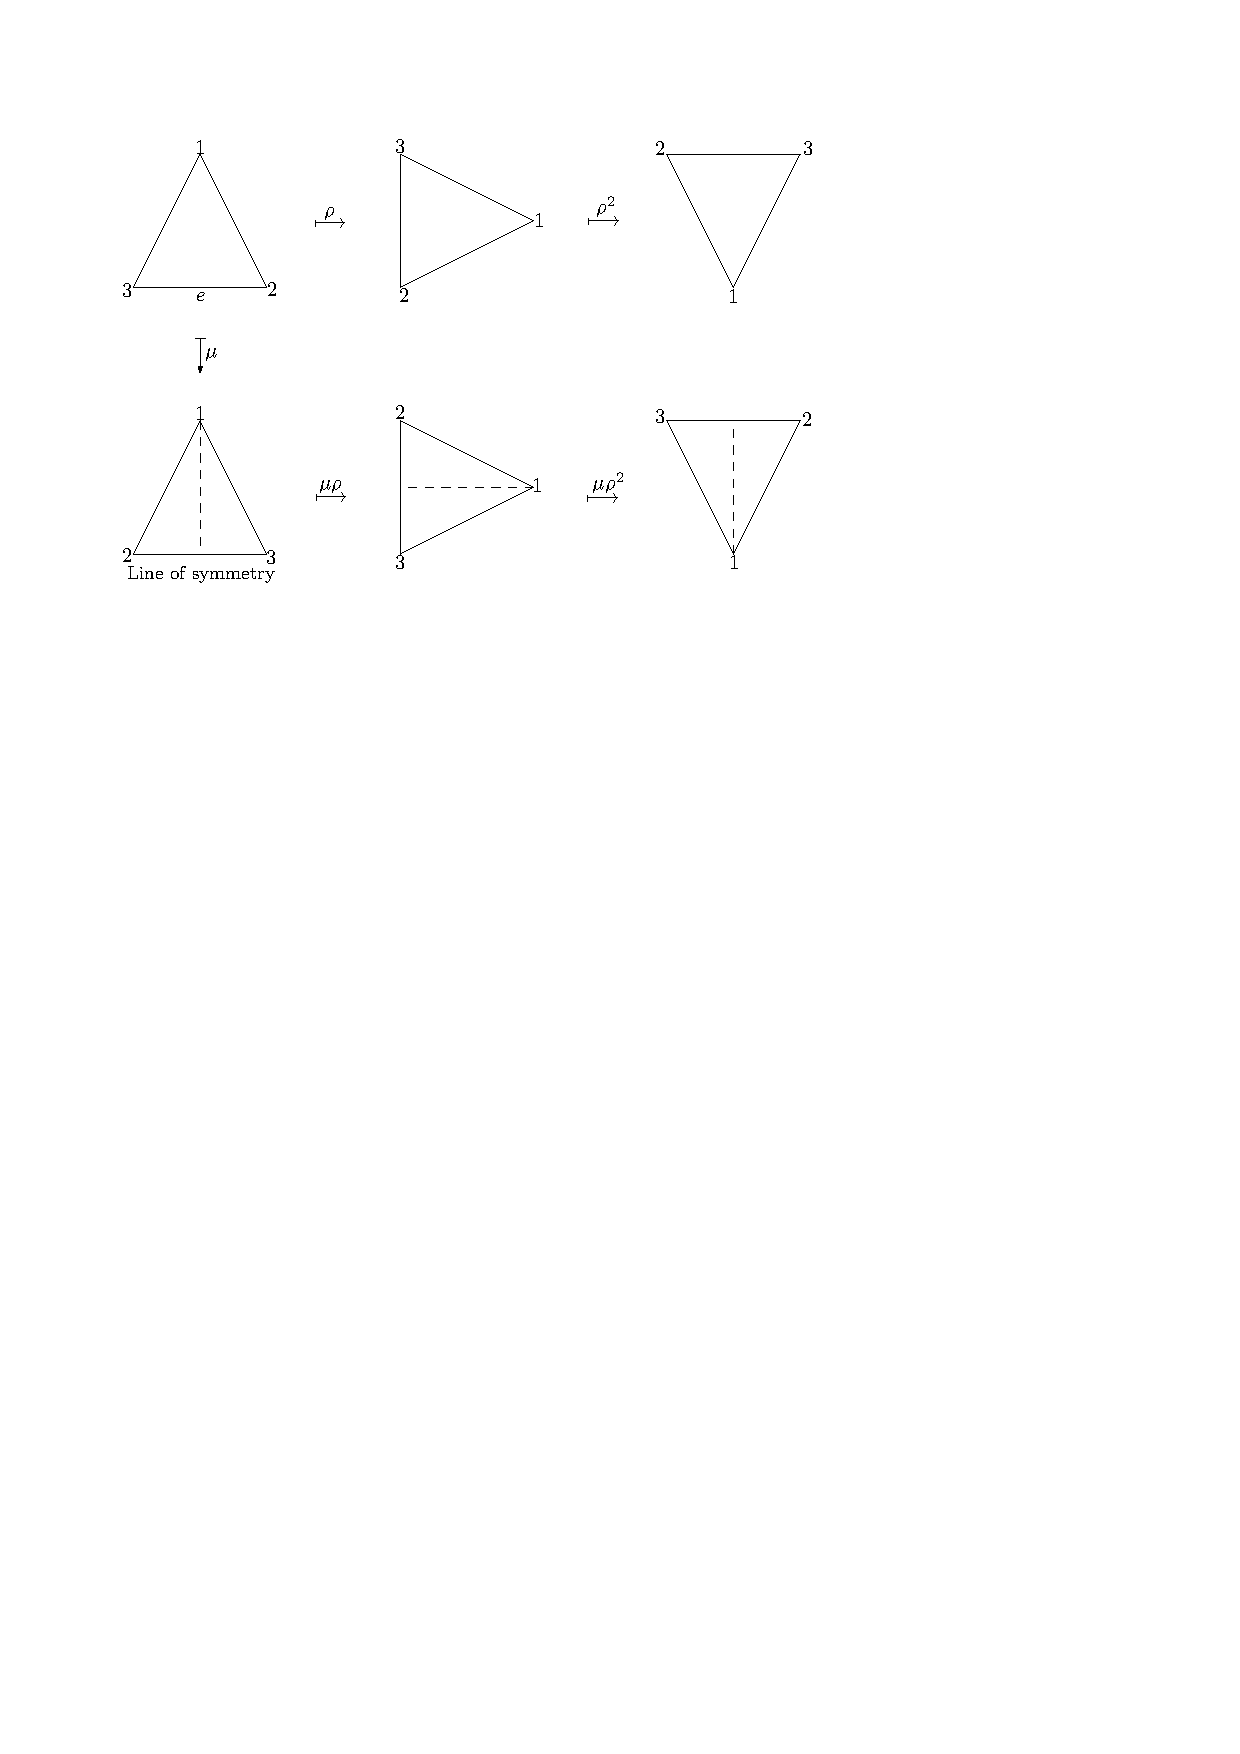
\includegraphics[width=0.7\textwidth]{./figures/d3.pdf}
    \caption{}
    \label{}
\end{figure}

The observed triangle is a geometric representation of \( D_{3} \). We can see that the order is given by \( |D_{3}|=|\{ e,\rho ,\rho ^2,\mu ,\mu \rho ,\mu \rho ^2 \}|=6 \), the same as \( S_3 \); however when observing \( D_{4} \) and \( S_{4} \), we notice that these are incapible of being isomorphic since they have different orders: \(|D_4|=|\{ e, \rho ,\rho ^2,\rho ^3,\mu ,\mu \rho ,\mu \rho ^2,\mu \rho ^3\} | =8 \) and \( |S_{4}|=|\{ e,\sigma ,\sigma ^2,\sigma ^3,\tau \sigma ,\tau \sigma ^2,\tau \sigma ^3,\tau ^2 \sigma , \ldots  \}| = 24 \). Interesting! It seems, from observation that while \( S_n \) follows the rule of order \( n! \), \( D_n \) follows the rule of order \( 2n \). Notice that the mappings that involve \( \mu  \) in \( D_{3} \) are all reflections on a different axis of symmetry, the axis of symmetry under \( e, \rho  \) and \( \rho ^2 \). We can thus imagine \( D_{3} \) as \( 2n \) due to the fact that it has \( n \) rotations, and therefore \( n \) axies of symmetry \( \implies n+n=2n \).\qed



\end{problem}

Something to note is that, as we increase in dimensionality (recall that \( D_n \) is restricted to \( n \)-gons in \( \mathbb{R}^2 \)), i.e., as \( n \) increases for \( \mathbb{R}^n \), then the order of the group has more and more complex reflections (\( \mu  \)s), which meet \( S_{n} \)'s order and even exceeds it. A general rule is: for \( \mathbb{R}^n \), \( |G|=2^n(n!) \). The number of rotations and reflections, however, can be infinite (for example consider the set of all symmetries of a circle). 

\begin{definition}[Linearity]
  Linearity of a bijective function is determined by the rule that \( \phi (v+w)=\phi (v)+\phi (w), \forall  v,w \in  \mathbb{R}^n \) and \( \phi (\lambda v) , \forall v \in \mathbb{R}^n, \lambda \in  \mathbb{R}\). Notice our \( v,w \) quantities are vectors and our \( \lambda  \) quantity is a scalar. 
\end{definition}


\begin{definition}[General and Special Linear Groups]

  Consider the symmetries of \( S=\mathbb{R}^n \) but restrict the set of bijections to be only those which are linear (as defined in the previous definition). This forms the group \( GL_n(\mathbb{R}) \), i.e., the group of \( n \times n \) matrices with nonzero determinant. Similarly, a special case is \( SL_n(\mathbb{R}) \), which is the special linear group which is the same as the general linear group except the determinant is specified to be \( 1 \). 
  
\end{definition}


\begin{definition}[Orthogonal Groups]
  An orthogonal group is a type of symmetric group that is the linear maps \( \Gamma : \mathbb{R}^n \to  \mathbb{R}^n \) that respect (preserve) distance.
\end{definition}

\subsection{Group Relations}

\begin{definition}[Subgroups]
  A subgroup of \( G \) is a subset \( H \subset G \) such that \( H \) is closed under the law of composition of \( G \) (i.e., \( \forall a,b \in  H ab \in  H \)) and \( \forall a \in  H \exists a^{-1} \in  H \) s.t. \( aa^{-1}=e \). 
\end{definition}


\begin{definition}[Generators and Generation]
  Group generation happens as a concequence of our definition of subgroups. Notice, that given \( H \le G \) (we use \( \le\) and \(\ge \) notation to indicate subgroup-ness) we can construct the smallest subgrop of \( G \) by taking the intersection of all subgroups of \( G \); notice that this intersection is indeed a subgroup as well. For generation of a group we want to take the samllest subset denoted \( S \subset G\) such that there exist a samllest subgroup that contains \( S \):
  \begin{displaymath}
    G_{smallest}=\bigcap_{H\le G; H\ge S} H
  \end{displaymath}
  we use the terminology that \( S= \langle S \rangle  \) is the generator of \( G \) if \( \langle S \rangle = G \).
\end{definition}

We can now use this bit of information to come up with a more formal definition of cyclic groups:

\begin{definition}[Cyclic Groups]
  A group is a cyclic group \( \iff \) all elements in the group are generated by a single element.
\end{definition}

\subsection{Homomorphisms}
\begin{definition}[Homomorphisms]
  If \( H \) and \( G \) are two groups, a homomorphism is given by \( \varphi : H \to  G \) as a map that respects the laws of composition in \( G \) and \( H \), i.e., \( \forall a,b\in H \),
  \begin{displaymath}
    \varphi (ab)=\varphi (a)\varphi (b).
  \end{displaymath}
  We can denote this using a commutative diagram,

  \[
    \begin{tikzcd}
G \times  G\arrow{r}{\varphi \times  \varphi } \arrow[swap]{d}{m_G} & H \times  H \arrow{d}{m_H} \\%
G \arrow{r}{\varphi}& H,
\end{tikzcd}
\] 
where \( m_G, m_H \) are the laws of compsoition for \( G,H \), respectively. What makes this diagram a homomorphism is thereby the very fact that it commutes. 
\end{definition}

Let's take two interesting cases: the inverse and the identity of a group under homomorphism: consider \( e_H \) and \( e_G \). By homomorphism, it must be the case that \( \varphi (e_He_G)=\varphi (e_H) \varphi (e_G) \), however, notice that since this is the identity, in order to preserve group structure, we result in the identity (\( e_H \) or simply \( e \)). if this is the case we can say \( \varphi (e_G)=e \) and \( \varphi (e_H)=e \), thus, \( \varphi (e_H)=e=\varphi (e_G) \). Similarly, take the inverse of some given \( a \in  G \), \( a^{-1} \in  G \), notice that \( \varphi (a^{-1})=\varphi (a)^{-1} \).

% ============================================================
% lecture_06
% ============================================================

\lecture{6}{category theory}

\section{Category Theory}

% Your notes here...

\subsection{Categories}

\begin{definition}[Category]
  A category \( \mathscr{C} \) is a collection of \textbf{objects}, such that:

  \begin{enumerate}[(i.)]
    \item for each pair of objects \( A,B\in  \text{Ob}(\mathscr{C} )   \);
    \item a collection of morphisms is given by \( \text{Mor}(A,B) \);
    \item there exists operation titled \textit{composition of morphisms} given by \[ \text{Mor}(A,B)\times \text{Mor}(B,C) \to \text{Mor}(A,C) \] such that \( f,g \mapsto g \circ f \);
    \item Category Theory Axioms: \begin{enumerate}
        \item every object \( A \) has an identity morphism \( \text{id}_A \in  \text{Mor}(A,A) \) such that \[ \forall f \in  \text{Mor}(A,B), \, f \circ \text{id}_A=\text{id}_B\circ f=f ;\]
        \item composition (of morphisms) is associative, i.e., \( (f\circ g)\circ h= f\circ (g\circ h) \).
    \end{enumerate}
\end{enumerate}

\end{definition}

We can think of categories and sets as, for the most part, the same thing, except for the fact that a category may include the category of all sets; this is where we deliniate sets and categories in order to avoid pesky paradoxes. 

Some examples of categories, for purposes of clarity:
\begin{enumerate}
  \item category of sets, \( \text{Mor}(A,B)= \) all maps \( A \to  B \)
  \item \( \text{Vect}_k \) as a fin. dim. vector space over \( k \), then \( \text{Mor}= \) linear maps
  \item groups, group homomorphisms 
  \item topological spaces, continuous maps
  \item and more...
\end{enumerate}

There exists a relationship called \textbf{isomorphism} not too dissimilar from group-theoretic isomorphisms. 

\begin{definition}[Isomorphism]
  \( f \in  \text{Mor}(A,B) \) is an \textit{isomorphism} if has inverse, i.e., \( \exists g \in  \text{Mor}(B,A) \) s.t. \( g \circ f =id_A \) and \( f \circ g =id_A \) \( \implies \text{if }\exists g \implies !\exists g \) and that \( \text{id}_A \) is an isomorphism. \( f \implies f^{-1} \) (\( g\equiv f^{-1} \\ \) )are both called isomorphisms, individually. 
  
\end{definition}
  Concequentially the automorphisms \( Aut(A) \) is always a group. 

sets :permutations, groups: automs, vec: invertible lin op. 

Isomorphic objects of \( e \) have isomorphic automorphic groups. Given \( f \in  \text{Mor}(A,B) \) as an isomorphism \( c_f:Aut(A) \to  Aut(B) \) which maps \( g \mapsto f \circ g \circ f^{-1} \). 

We may define sum, product, and quotient objects in categories. Consider a product \( A\times B \coloneqq \mathcal{C} \) of objects \( A,B \in  \mathscr{C} \) characterized by \( \mathcal{P} \) projects \( \pi_1 \in \text{Mor}(\mathcal{P},A), \pi_{2}\in \text{Mor}(\mathcal{P}, A) \) s.t. \( \forall  \) object \( T \), \( \forall f_{1}\in \text{Mor}(T,A), f_{2}\in \text{Mor}(T,B), \, \exists \) unique \( f \in \text{Mor}(T,\mathcal{P}) \) s.t. \( \pi_{1} \circ f =f_1, \, \pi_{2}\circ f=f_{2} \). 

\begin{figure}[ht]
    \centering
 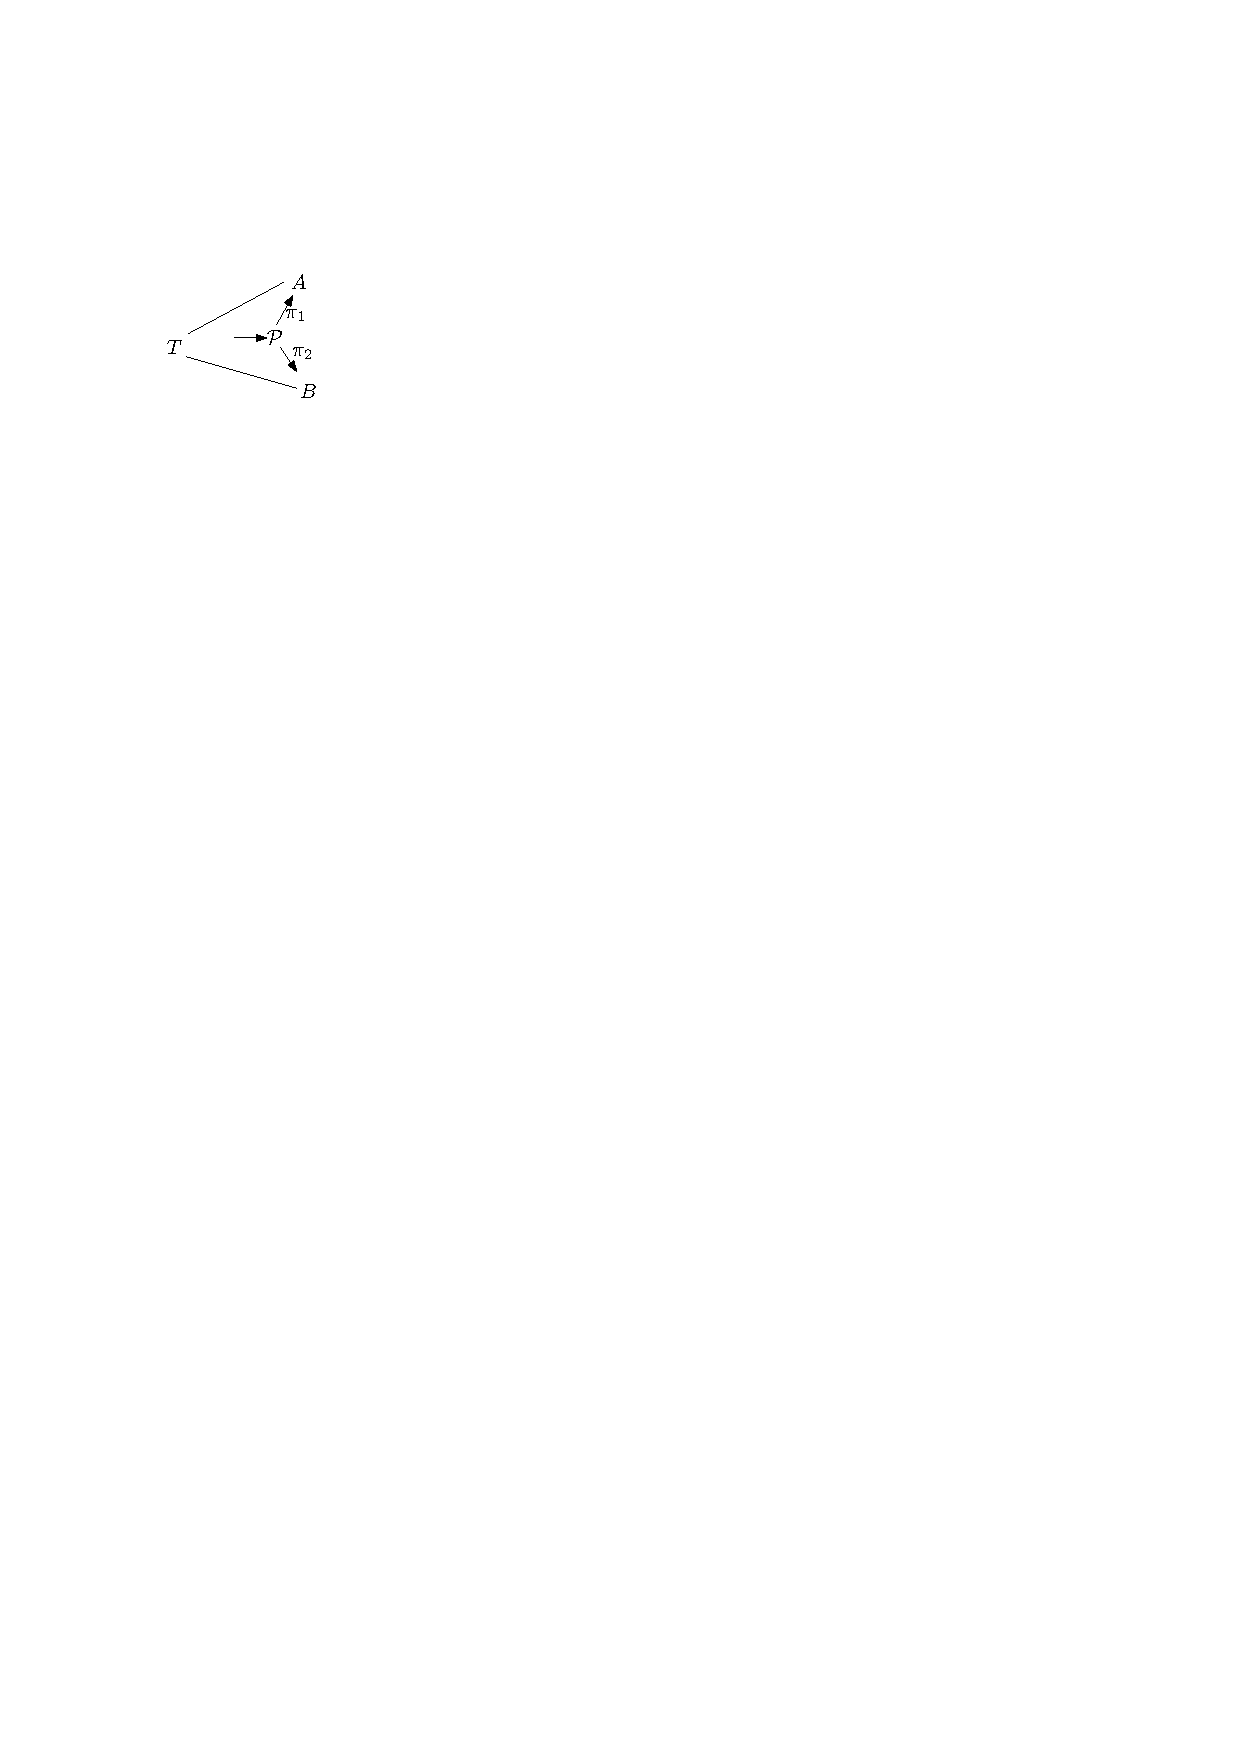
\includegraphics[width=0.2\textwidth]{./figures/tcat.pdf}
    \caption{}
    \label{fig:tcat}
\end{figure}

\begin{definition}[functor]
  \( C,D \) categories, a (\textit{covariant}) functor \( F:C \to  D \) is an assigment:
  \begin{enumerate}
    \item for every object \( X \) of \( C \) an object \( F(X) \) of \( D \)
    \item for each morphism \( f \in  \text{Mor}_C(X,Y) \), a morphism \( F(f) \in  \text{Mor}_D(F(X),F(Y)) \) s.t. \begin{enumerate}
        \item \( F(id_X)=id_{F(X)} \)
        \item \( F(g \circ f)= F(g)\circ F(f) \)
    \end{enumerate}
  \end{enumerate}
\end{definition}

Consider Forgetful functors , on a vector space over k given vector sace \( V \) \( F: Vect_k \to Vect_k \)objects: \( W \mapsto Hom(V,W) \) lin. maps \( V \to  W \), morphism \( f: W \to  W'\implies?? \)

Anywhos. He's going on about linear maps as morphisms for categories and functors but I don't care all that much at the moment. As a functor \( F : \text{Vect}_k \to  \text{Vect}_k \) can be shown as \( Hom(V, \circ) \). What the mell does obj. \( V \mapsto V_{\mathbb{C}}=V\oplus iV\)

\begin{definition}
  A \textit{contravariant functor} \( F : C \to D \) is the same except reverses direction of morphism:
  \begin{displaymath}
    f \in  \text{Mor}_C(X,Y) \mapsto F(f) \in  \text{Mor}_D(F(Y),F(X)) \mid  F(g\circ f)=F(f) \circ F(g).
  \end{displaymath}
\end{definition}

So for example, consider \( V \to V^* \) s.t. \( f \in  Hom(V,W) \mapsto f^* \in  Hom(W^*,V^*) \). 

\begin{definition}
  Given two functors \( F,G : \mathscr{C} \to  \mathscr{D} \) a natural transformation \( t \) from \( F \) to \(G\) is the data \( \forall X \in  Ob(\mathscr{C}) \), a morphism \( t_X \in  \text{Mor}_{\mathscr{D}}(F(X),G(X)) \) s.t. 

 \[
 \forall  X, Y \in  Ob(\mathscr{C}), \forall f \in  \text{Mor}_{\mathscr{C}}(X,Y), \]
 \[
\begin{tikzcd}
F(X) \arrow{r}{F(f)} \arrow[swap]{d}{t_x} & F(Y) \arrow{d}{t_y} \\%
G(X) \arrow{r}{G(f)}& G(Y)
\end{tikzcd}
.\]
  
\end{definition}

\begin{definition}[Bilinear forms]
  A \textbf{\textit{bilinear form}} on a vector space \( V \) over a field \( k \) is a map \( b:V \times V \to  k \) (this is to say we take \( (v,w)\mapsto b(v,w) \)) that is linear in each variable, i.e., \( \forall u,v,w \in  V, \, \lambda \in  k, b(\lambda v,w)=b(v,\lambda w)=\lambda b(v,w) \) ("multiplied" on both sides separately). 
\end{definition}

\begin{definition}[symmetric]
  Say \( b \) is symmetric if \( b(v,w( = b(w,v) )) \forall v,w \in  V \) and is skew symmetric if \( b(v,w)=-b(w,v) \).
\end{definition}

I have mentally clocked out, I spent last night and this morning going over the notes for today and ngl i understood it better before he started explaining it 

AWWWWWW 

\[
  \begin{tikzcd}
    A \arrow{r}{f} \arrow[swap]{dr}{g\circ f} & B \arrow{d}{g} \\%
& C
\end{tikzcd}
.\]

% ============================================================
% lecture_07
% ============================================================

\lecture{7}{lec15}

\section{Lecture 15}

% Your notes here...
%

\subsection{bilinear forms}

\textbf{Bilinear forms} on fin. dim. vec. space \( V \) over \( k \) for
\[ b: V \times  V \to k \longleftrightarrow  \varphi _b \in  \text{Hom}(V,V^*)\]
which gives an isom. \( B(V) \cong \text{Hom}(V,V^*) \) (\( \varphi  _b (v)=b(v,\cdot) \))

Say be in non degenerate if \( \varphi_b  \) is injective. 

In a basis \( (e_{1},\ldots e_n) \) of \( V \), rep. \( b \) by a mat. \( A \) w ent \( a_{ij}=b(e_i,e_j) \) .

\[
  b(\sum_i x_ie_i,\sum_jx_je_j) = \displaystyle\sum_{i,j}^{ a_{ij}x_iy_j}=X^{\perp}Ay
.\] 

where col. vectors are \( X \) and \( y \) that correspond to the summations in \( b \). 


Something something
\begin{enumerate}[i.]
  \item \( b \) is symm. \( \iff \) \( A \) is symm. (\( b(v,w)=b(w,v) \iff A^{\perp}=A, a_{ij}=a_{ji} \))
  \item \( b \) is nondegenerate \( \iff \) \( A \) is invertible. 
\end{enumerate}


 "Two vectors paired together to zero"

\begin{definition}[Orthogonality]
  If \( S \subset V \) is a subspace of \( V \), \( b:V\times V \to k \) w/ is bilinear form, the \textbf{orthogonal compliment} is \( S^{\perp}=\{v \in  V \mid  \forall w \in  S, b(v,w)=0 \} \)
\end{definition}

Beware: if b is skew symmetric or symm. then \( (*)\iff \forall w \in  S, b(w,v)=0 \), otherwise (not skew symm or symm) we we have a left orthogonal and a right orthogonal (such that they are not the same), buttttt we want to have them be equal so we just will ignore this for now lol. 

\begin{lemma}
  If \( b \) is nondegenerate then \( dim(S^{\perp})=dim(V)-dim(S) \), else ineq. 
\end{lemma}

\begin{proof}
  
  \begin{displaymath}
    S^{\perp}=      \text{ker} \left( V \to  S^*, \, (v \mapsto \varphi _b(v)_{\mid S} =b(v,\cdot)_{\mid S}) \right)
  \end{displaymath}
  which is the composition of \( \varphi _b V \to  V^* \) and restriction \( r: V^* \to  S^* \) and \( l\mapsto l_{\mid S} \) which is surjective. So by rank thm. \( \text{dim}S^{\perp} \text{dim}V-\text{rank}(r \circ \varphi _b ) \le \text{dim}(S^*)=\text{dim}(S) \) is \( b  \) is nondegenerate then \( r \circ \varphi _b \) is surjective so \( rk=\text{dim}S \).
\end{proof}


Note: write less don't merely copy. Perhaps only do definitions and misc. info? proofs seem to be something you can go over post lecture, just try to understand for now. 


Ex: \( V=\mathbb{R}^n \) with standard dot prod. so \( b(v,w) = \sum v_i w_i \) Then \( V= S \oplus S^\perp \)


\begin{definition}[Inner Product Spaces]
  An \textbf{inner product space} is a vector space \( V \) over \( \mathbb{R} \) together with a symmetric positive definite bilinear form \( \langle *,*\rangle: V \times V \to  \mathbb{R} \).
\end{definition}

\begin{definition}[ips symmetric]
  \( \langle u,v \rangle =\langle v,u \rangle \)
\end{definition}

\begin{definition}[positive definite]
  \( \langle u,u \rangle \ge  0 \forall u \in  V \), and \( \langle u,u \rangle=0 \iff u=0 \).
\end{definition}

\begin{definition}[norm]
  The \textbf{norm} of a vector is \( | | v | | = \sqrt{\langle v,v\rangle}  \). \(v,w \in V \) are orthogonal if \( \langle v,w \rangle =0 \). 
\end{definition}

\begin{theorem}[Cauchy-Scwartz inequality]
  yk what this is lol, just do it with norms \( |\langle u , v \rangle | \le | | u | | | | v | | \)
\end{theorem}

\begin{theorem}
  Every finite dim inner product space \( / \mathbb{R} \) has an ortho basis.
\end{theorem}

\[
  \frac{\mathrm{d/V}}{\mathrm{dx}} 
.\]

% ============================================================
% lecture_08
% ============================================================

\lecture{8}{lec16}

\section{Orthogonal adjoint operators and Hermatians}

% Your notes here...




\begin{definition}
  \( T \) is self-adjoint if \( T^* = T \), i.e., 
  \begin{displaymath}
    \langle T u , v \rangle = \langle u,Tv \rangle 
  \end{displaymath}
  so \( \mathcal{M}(T) \) in an orthogonal basis is symmetric (\( \mathcal{M}_{ij}=\mathcal{M}_{ji} \)). 
\end{definition}



\begin{theorem}[spectral thm]  
  If \( T : V \to  V  \) is self adjoint then \( T \) is diagonalizable, with real eigenvalues. Even more, T can be diagonalized in an orthogonal basis of \( ( V, \langle \cdot , \cdot  \rangle ) \)!  

\end{theorem}

% ============================================================
% lecture_09
% ============================================================

\lecture{9}{Hermitians, \( \CC\)-spectrals, etc.}

\section{Hermitian inner products}

We now wish to real with inner products on complex vector spaces (as opposed to our previous study on \( \mathbb{R} \)). Hermitian inner products are \( \CC \)-linear, i.e., conjugate-linear in one of the inpts. 

\begin{definition}{Hermitian forms}{hermforms}
A \textbf{Hermitian form} on a \( \CC \)-vector space \( V \) is \( H: V\times V \to  \CC[] \) s.t.
\begin{enumerate}
  \item \( H \) is \textbf{\textit{sesquilinear}}
    \begin{itemize}
      \item \( H(u,v+w)=H(u,v)+H(v,w)\)
      \item \( H( u, \lambda v) =\lambda  H (u,v)\)
      \item however, \( H(\lambda u, v)= \overline{\lambda }  H(u,v) \), where our \( \overline{\lambda }  \) is our complex conjugate (just \( \overline{z}  \) really). 
    \end{itemize}
  \item \( H \) conjugate symmetric \( H(u,v)=\overline{H(v,u)} \implies H(u,v) \in  \mathbb{R} \)
\end{enumerate}
\end{definition}

\begin{definition}{Hermitian inner products}{herminner}
  A hermitian inner product on \( V \) is a positive definite  \(  (H(u,u)\ge 0 \forall u \neq 0) \)
\end{definition}

\begin{mybox}{blue}{Remark 1}
  \[
    \varphi _H : V \to  V^*, \, u \mapsto H(u,\cdot )
  \]
  where \( H \) is \( \CC \)-linear \( V \to  \CC \) and \( H \) is linear in the second input. We say \( \varphi  \) is a \textbf{\textit{complex antilinear}} map, and \( (\varphi (\lambda  u ) = \overline{\lambda } \varphi (u) ) \).
\end{mybox}

In the case that \( H \) is positive def. \( \implies \) nondegenerate \( \forall (u \neq 0)\in  V , \varphi _H(u)=H (u,\cdot )\neq 0\). When we are given a subspace \( S \subset  V \), it must be orthogonal, 
\[ S^\perp = \{v \in  V \mid H(v,w)=0 \forall w \in  S\}   \]
s.t. it is a subspace. Of course, as with any finite dimensional conjugate \( \text{dim}V<\infty \), we have \( (S^{\perp})^\perp \). Continuing on, we note that when \( V = S \oplus S^\perp \), \(S \cap S^\perp = \{0\} \), \[
  u \in  S \cap S^\perp \implies H(u,u) \text{ where the first \( u \in  S\), and the second \( u \in  S^\perp \)} =0 \implies u=0,
\] 
so \( \text{dim}S^\perp = \text{dim} V - \text{dim}S \)

\begin{theorem}{Th}{t}
  \( V \) admits an orhtogonal basis in \( \CC\). The proof is the same as in \( \mathbb{R} \). 
\end{theorem}

\begin{definition}{}{}
  An \textbf{orthonormal basis} of \( (V,H) \) is a basis \( \{e_i\}   \) s.t. 
  \begin{displaymath}
    H(e_i,e_i)=\|e_i\|^2 =1, \, H(e_i,e_j)=0 \forall i\neq j, e_i \perp e_j. 
  \end{displaymath}
  
\end{definition}

some other stuff


...
...
So, in matrix form, \( H(z,w)=\overline{z}^{\text{T}}w =z^*=(\overline{z}_{1}\ldots \overline{z}_n) \) as conjugate transpose. 

Consider fourier series as a (sorta-kinda) example of \( V=C^{\infty} (S^1,\CC) \) w/ is infinitely differentiable \( S^1=\mathbb{R}/\mathbb{Z} \to  \CC, (\iff 1)\)-periodic functions \( \mathbb{R} \to  \CC \). \( L^2 \)-inner product, \[
  H(f,g)=\int_{S^1}\overline{f(t)} g(t)dt = \int_0^1 \overline{f(t)} g(t)dt\]
  and 
  \[
    H(f,f) = \int _0^1|f(t)|^2 > 0\,  \text{ if } f\neq 0
  .\] 
  Note that then \[ f_n(t) =e^{2 \pi  i nt} = \cos (2 \pi  nt) + i \sin  (2 \pi  nt), n \in  \mathbb{Z}\] is orthogonal! So, \( H(f_n,f_m)=\delta _{n,m}  \). 


  \begin{definition}{}{}
 We let \( V \) be a complex space, \( H \) a Hermitian inner product, and \( T:V \to  V \) a linear operator.
  \begin{displaymath}
    \text{the adjoint of } T \text{ is } T^* : V \to  V \text{ s.t. } H(T^*v,w)=H(v,Tw) \forall v,w \in  V
  \end{displaymath}
  \[
    (\iff H(Tv,w)=H(v,T^*w))
  .\] 


\end{definition}{}{}
Some immediate concequences:
\begin{itemize}
  \item \( T \) is \textit{self-adjoint} if \( T^*=T \)
  \item \(  T \) is \textit{unitary} if \( H(Tv,Tw)=H(v,w) \)
  \item \( T \) is normal if \( TT^*=T^*T \)
    unitary operators form a group (omg!) \( U(V)=U(V,H) \subset \Aut(V) = \text{GL}(V) \), \( U(n) \subset  \text{GL}(n,\CC) \), e.g., \( U(1)=S^1=\{z \mid  |z| = 1\} \subset  \CC[*]  \). 
\end{itemize}





\begin{mybox}{orange}{Proposition 1}
    in an orthonom. basis \( \mcM (T^*) = \mcM (T)^*=\overline{\mcM(T)^t}  \) so \( H(Tv,w)=(\mcM v )^*w = v^* (\mcM^* w)=H(v,T^*w) \), self-adjoint operators \( \leftrightarrow \) Hermitian matricies 

\end{mybox}


\begin{definition}{Complex spectral theorem}{compspecthr}
  put it here 
\end{definition}

proof goes here

in such a basis \( \mcM (T) = \begin{pmatrix} \lambda_1 & \, & 0 \\ \, & \ddots& \, \\ 0 & \, & \lambda_n \end{pmatrix}  \)


\subsection{some number theory (non-degenerate symmetric bilinear forms)}

this u can go over later via the notes just put it in here





\begin{definition}{}{}
test
\end{definition}

% ============================================================
% lecture_10
% ============================================================

\section{test}

lalalal


% Your notes here...

\end{document}
